LFV cuts:
preselection
same preselection cuts for 8 and 13 TeV LFV
use ak5PFJets at 8 TeV, ak4PFJets at 13 TeV (ak4pfjets more stable with respect to pileup)
require opposite sign leptons
clean jets (dR > 0.4)
veto extra muons
	8 TeV:  passing RelPFIsoDB < 0.15 and pt> 5 GeV (mutauhad) or pt > 7, PFIDLoose
	13 TeV: passing RelPFIsoDB < 0.15 and pt> 5 GeV (mutauhad) or pt > 10 GeV and RelPFIsoDB < 0.25
	RelPFIsoDB: sum charged + max(0, sum neutral + sum em = 0.5 sum PU)/ptmu < 0.15
	PFIDLoose: use all PF muons
veto extra electrons
	8 TeV: CicTightIso Pt  10 GeV
	13 TeV: RelPFIsoDB < 0.3 (mutauhad) or RelPFIso(EA) < 0.5 with Pt > 10 GeV
veto extra tuas
	8 TeV: Pt > 20 GeV
	13 TeV: Pt > 20 GeV
muon
	8 TeV: PFIDTight, pt> 30 GeV (25 for etau), eta < 2.1, RelPFIsoDB < 0.12
	13 TeV: TightID, pt > 25 GeV, eta < 2.1, RelPFIsoDB < 0.15
	PFIDTight: https://twiki.cern.ch/twiki/bin/view/CMSPublic/SWGuideMuonId#Tight_Muon
	Efficiency corrections applied (from tag and probe)
	cone of 0.4
electron
	8 TeV: PFIDLoose, pt > 10 GeV, eta < 2.3, DZ < 0.2, RelPFISoDB < 0.12
	13 TeV: Pt > 15, eta < 2.3, MVA Electron ID 90\% (non triggering), RelPFIsoEA<0.1
	Cone of 0.3 for RelPFIsoDB
	RelPFIsoEA (PU = rho * effective area)
	rho = average PU density per area in phi-eta plane
tau
	8 TeV: PFTauHPS, tightIsoHits3, Pt > 30 GeV, eta < 2.3, AntiElectronLoose, AntiMuonTight2
	13 TeV: PFTauHPS, DeltaBetaCorr3Hits, AntiElectronMediumMVA5, AntiMuonTight3
	iso at 8 TeV: 0.5 cone, isolation pt charged + max(pt gamma-deltaBeta, 0)
	deltaBeta = 0.46*pt charged (dz > 0.2 cm)
	iso at 13TeV: 0.4 cone
	8 TeV and 13 TeV: tight sum of less than 0.8 GeV
Bjet veto mutaue (30 GeV), for 8 and 13 TeV (CSV)

Systematics:
Muon trigger/id/iso: tag and probe
hadronic tau efficiency: 
cross section uncertainties: increased from 8 TeV to 13 TeV because of less studies

\section{Background Estimation}

\subsection{Monte Carlo Samples Used: This section will simply list the Monte Carlo samples used, in contrast with the Monte Carlo Generation section which will list the different Monte Carlo generator techniques.}
8 TeV:
The dominant backgrounds are estimated with data  while the less significant
backgrounds are estimated with simulations.  The largest backgrounds come from $Z \to \tau \tau$
and from jets faking leptons in $W+jets$ and QCD multi-jet events. The $Z \to \tau \tau$
background is estimated using an embedding technique in which simulated tau decays replace
the muons in $Z \to \mu \mu$ data. The misidentified lepton rates are measured in an independent data
set and then applied to control regions to estimate the background.



13 TeV:
The background contribution from $\cPZ \rightarrow \Pgt\Pgt$ is estimated with simulation. The simulated events are corrected for residual discrepancies between data and simulation. These discrepancies, which are related to the lepton triggering, identification, and isolation, are determined from the tag-and-probe technique in $\cPZ \rightarrow ll$ data~\cite{Chatrchyan:2012xi, Khachatryan:2015hwa}. The background contribution coming from SM H decays in the $H \rightarrow \Pgt\Pgt$ channel is
estimated with simulation. This background is suppressed by the kinematic selection criteria
and peaks below 125 $GeV$. The $W$ leptonic decay from  $t\bar{t}$ produces opposite-sign dileptons and $MET$. In the $\mu \tau_{e}$ channel this background is estimated with simulated $t\bar{t}$
events using the shape of the $M_\text{col}$ distribution from simulation and a data control region for
normalization. The control region is the  2-jet selection but with the additional requirement that
at least one of the jets is b-tagged in order to enhance the $t\bar{t}$ contribution.
Other backgrounds come from $WW$, $\cPZ\cPZ$, $W\gamma$ and single
top-quark production. Each of these is estimated with simulation.
\subsection{QCD Estimation}
\subsection{Tau Embedding}
8 TeV pas
The  $Z \rightarrow \tau \tau$  background is estimated using a particle flow embedding technique.
%~\cite{CMS_AN_2013-073}. 
A sample of $Z \rightarrow \mu \mu$ events is taken from data using a loose selection. The muons are then replaced
with simulated tau decays reconstructed with the particle flow algorithm. Thus the key features of the event topology such as the
jets, missing energy and underlying event are taken directly from data with only the tau decays being simulated. The normalization
of the sample is from the simulation expectation. The technique is validated by comparing identification efficiencies
estimated with embedded decays to those from  simulated $Z \rightarrow \tau \tau$ decays. It is found that the muon and hadronic
tau efficiencies are well reproduced. There are small differences in the the electron identification efficiency.
 The differences are
%~\cite{CMS_AN_2013-073} 
understood to be a consequence of
the selective readout of the ECAL and corrections are applied for this.
\subsection{Fake Rate Method}
8 TeV:


Leptons can arise from misidentified jets  from $W\mathrm{+jets}$ and QCD multi-jet events. This background is estimated using a data based method.
%~\cite{CMS_AN_2012-120}. 
It is employed slightly differently in the
two channels. The technique is shown schematically in Table~\ref{tab:fakeratediagram}.
The difference in the two channels is how the selection requirements are altered to define regions III and IV.
In $H \rightarrow \mu \tau_{e}$ region I is the signal region in which an isolated muon and an isolated electron is required.
Region III is a data sample in which all the analysis selection criteria are applied except that
one of the leptons is required to be not-isolated, so that there are two components;  isolated muon plus not-isolated
electron events, and also isolated electron plus not-isolated muon events.

\begin{table}[hbtp]
 \begin{center}
 \caption{Schematic to illustrate the application of the method used to estimate the misidentified lepton background. Samples
are defined by the charge of the two leptons and by the selection requirements on each. The selection requirement and charge requirement
is altered on the second lepton to define four regions.}
  \label{tab:fakeratediagram}
  \vspace{0.1in}
  \begin{tabular}{|l|c|c|} \hline
                                                   & Opposite Sign leptons &  Same Sign leptons     \\ \hline
Selection(lepton1), Selection$^{*}$(lepton2)          & Region III            &  Region IV             \\ \hline
Selection(lepton1), Selection(lepton2)              & Region I              &  Region II             \\ \hline
  \end{tabular}
 \end{center}
\end{table}



\begin{figure*}[hbtp]\begin{center}
%\includegraphics[width=0.48\textwidth]{plots/mue_likesign_regionII.pdf}
%\includegraphics[width=0.48\textwidth]{newplots/fakesEle.pdf}
%\includegraphics[width=0.48\textwidth]{plots/muhad_likesign_regionII.pdf}
%\includegraphics[width=0.48\textwidth]{newplots/fakesMu.pdf}
\caption{Left)  $M_{collinear}$ for the $H \rightarrow \mu \tau_{e}$ same sign isolated $e$ or $\mu$ plus isolated $\mu$ or $e$ sample (region II).
         Right) $M_{collinear}$ for the $H \rightarrow \mu \tau_{had}$ same sign isolated muon plus tight-isolated tau (region II). }
\label{fig:samesign_fakes}\end{center}\end{figure*}


These samples are dominated by $W\mathrm{+jets}$ and QCD multi-jets but with small backgrounds from $WW,ZZ$  that are subtracted using
simulation expectations. The misidentified  muon background in region I is then estimated by multiplying the event yield in region III by a
factor $f_{\mu}\cdot\epsilon_{trigger}$, where $f_{\mu}$ is the ratio
of not-isolated to isolated muons. It is computed in an independent data sample $\cPZ(\mu \mu) + (X=\mu)$
\begin{equation*}
f_{\mu}=\frac{ N_{events}(\cPZ(\mu \mu) + \mu_{isolated}) }{N_{events}(\cPZ(\mu \mu) + \mu_{not-isolated}) }.
\end{equation*}
in bins of muon $p_{T}$ and $\eta$. A correction $\epsilon_{trigger}$ is made to
account for the difference in trigger efficiency for selecting the isolated electron plus not-isolated
muon versus selecting the isolated electron plus isolated muon. It is computed by selecting data
in an independent single electron triggered data sample, applying the full event selection and then taking the
ratio of the number of events that pass the electron-muon cross-trigger from the isolated versus
not-isolated sample. The misidentified electron background is computed in exactly the same way.
The technique is validated by using a like-sign rather than opposite-sign data sample in
the same way as shown schematically  in Table~\ref{tab:fakeratediagram}. Like sign leptons are chosen rather than opposite sign.
Figure~\ref{fig:samesign_fakes} shows the measured  versus predicted by simulation $M_{collinear}$ distribution for the like sign control region. The agreement is very good.




In the $H \rightarrow \mu \tau_{had}$ channel tau leptons can be misidentified jets arising from a number of sources. Predominantly  $W\mathrm{+jets}$ and QCD multi-jet events, but also
 $\cPZ(\mu \mu) \mathrm{+jets}$ , $t\bar{t} \mathrm{+jets}$. The misidentification rate $f_{\tau}$ is measured in $\cPZ(\mu \mu) +X=(\tau)$ events. It is
defined as
\begin{equation*}
f_{\tau}= \frac{N_{events}(\cPZ(\mu \mu) +X=(\tau, ID+tight-isolated))}
               {N_{events}(\cPZ(\mu \mu) +X=(\tau, ID+loose-isolated))}.
\end{equation*}
The denominator is the number of events with an object identified as a $\tau$
except that the requirement on isolation is loosened. The
numerator is the number of events where the normal tau isolation (tight-isolated) requirement is made.
The misidentification rate  measured in  $\cPZ(\mu \mu) +X=(\tau)$ data is checked by comparing to that
measured in $\cPZ(\mu \mu) +X=(\tau)$ simulation and found to be in good agreement.
The measured misidentification rate is then used in the same way as previously described, and illustrated schematicallyin Figure~\ref{tab:fakeratediagram}. In this case region I, the signal region is the baseline
event selection with both an isolated tau and an isolated muon. Region III comprises the baseline
selection with an isolated muon and a {\it loose-isolated\&not-tight-isolated} tau  requirement.
This region is dominated by $W\mathrm{+jets}$ and QCD multi-jet background and there good agreement between the
data and the expected yields from simulation. The isolated muon plus
{\it loose-isolated\&not-tight-isolated} tau  region is then used  to estimate the misidentified lepton  background using the following relation:

\begin{equation*}
\frac{N_{events}(\tau_{tight-isolated})}
     {N_{events}(\tau_{loose-isolated.\&.not-tight-isolated})}
= 
\frac{f_{\tau}N_{events}(\tau ID)}
     {(1-f_{\tau})N_{events}(\tau ID)}.
\end{equation*}
Hence the background in the signal region (region I) is given by
\begin{equation*}
N_{events}(\tau_{ tight-isolated})= 
\frac{f_{\tau}}
     {(1-f_{\tau})}N_{events}(\tau_{loose-isolated.\&.not-tight-isolated}).
\end{equation*}

The procedure can be validated with like sign $\mu\tau$ events. Figure~\ref{fig:samesign_fakes}
shows the excellent agreement between data and simulation for the like sign samples.
As an additional test, the method is tested on opposite sign $\mu\tau$ events, with tight
isolation applied to the tau, after the pre-selection and without the requirements on the kinematic variables.
Again there is excellent agreement between  data and simulation for this region.

The method assumes that the misidentification rate in $\cPZ(\mu \mu) +X=(\tau)$ events is the same as
for $W\mathrm{+jets}$ and QCD processes. To test this assumption the misidentification rates are measured in a QCD data control
sample. They are found to be consistent, but slightly lower. A conservative 30\% uncertainty is assigned.
Finally as a cross-check the study has been performed also as a function of the number of jets in the event and similar agreement found.


13 TeV:
The largest backgrounds come from $\cPZ \rightarrow \Pgt \Pgt$ and from misidentified leptons in $W$+jets and QCD multijet production. The contribution of the misidentified lepton background is estimated using data, while the remaining backgrounds are estimated using simulation.
The simulated backgrounds are normalized by applying a scale factor equal to the ratio of the observed luminosity in data to the effective luminosity of the simulated sample.


Reconstructed leptons can arise from misidentified jets in $W$+jets and QCD multijet processes.
This background is estimated with data. A sample with similar kinematic
properties to the signal sample but enriched in $W$+jets and QCD multijets
is defined. Then the probability for objects to be misidentified as leptons is measured
in an independent data set, and this probability is applied to the enriched sample to
compute the misidentified lepton background in the signal region.
The technique is shown schematically in Table~\ref{tab:fakeratediagram} in which four regions
are defined including the signal and background enriched regions (I and III) and two control regions (II and IV) used for validation
of the technique. It is employed slightly differently in the
$H \rightarrow \mu \Pgt_{e}$ and $H \rightarrow \mu \tauh$ channels because
the lepton isolation requirements used to define the enriched regions in each channel
are slightly different.

In the $H \rightarrow \mu \Pgt_{e}$ channel, region I is the signal region in which an isolated $\mu$ and an isolated $e$ are required.
In region III all the analysis selection criteria are applied to the data sample except that
one of the leptons is required to be not-isolated. This creates a misidentified lepton rich region. There are two types of events in this region: events with an
isolated $\mu$ and not-isolated $e$ events, as well as events with an isolated $e$ and not-isolated $\mu$ events. There is negligible number of signal events in region III. Regions II and IV are data samples formed with the same selection criteria as regions I and III, respectively, but with same-sign rather than opposite-sign leptons. The kinematic distributions of the same-sign samples are very similar to the opposite-sign samples

\begin{table}[hbt]
 \centering
 {
 \renewcommand{\arraystretch}{1.1}
 \caption{Definition of the samples used to estimate the misidentified lepton ($\ell$) background. They
are defined by the charge of the two leptons and by the isolation requirements on each.}
  \label{tab:fakeratediagram}

  \begin{tabular}{c|c}
  Opposite sign leptons & Like sign leptons \\
  \hline
% \rule[-5pt]{0pt}{20pt}
\textbf{Region I}              &  \textbf{Region II}             \\ \hline
$\ell^{\pm}_{1}$(isolated)  &  $\ell^{\pm}_{1}$(isolated)             \\
$\ell^{\mp}_{2}$(isolated)  &  $\ell^{\pm}_{2}$(isolated)             \\

\hline \hline
% \rule[-5pt]{0pt}{20pt}
\textbf{Region III}           &  \textbf{Region IV}             \\ \hline
$\ell^{\pm}_{1}$(isolated)  &  $\ell^{\pm}_{1}$(isolated)             \\
$\ell^{\mp}_{2}$(not-isolated )  &  $\ell^{\pm}_{2}$(not-isolated)             \\
\hline
  \end{tabular}
}
\end{table}

The sample in region III is dominated by $W$+jets and QCD multijets but with small
contributions from $WW,\cPZ\cPZ$ and $W\cPZ$  that are subtracted using
simulation. The misidentified  $e$ background in region I is then estimated by multiplying the event yield in region III by a
factor $f_{e}$, where $f_{e}$ is the ratio
of not-isolated to isolated $e$'s. It is computed in an independent data sample $\cPZ \rightarrow \mu \mu + X$, where $X$ is an object identified as a $e$, in bins of $p_{T}$ and $\eta$.
\begin{equation}
f_{e}=\frac{ N_{events}(Z \rightarrow \mu \mu + e_{isolated}) }{N_{events}(Z \rightarrow \mu \mu + e_{non-isolated}) }
\end{equation}
The $\cPZ \rightarrow \mu \mu + X$ sample is corrected for contributions from $WW,\cPZ\cPZ$ and $W\cPZ$ using  simulated samples.
The misidentified $\mu$ background is computed in exactly the same way.
The technique is validated by using the  same-sign data from regions II and IV
as shown schematically  in Table~\ref{tab:fakeratediagram}.
In Fig.~\ref{fig:samesign_fakes}(left) the observed data yield in region II is compared
to the estimate from scaling the region IV sample
by the measured misidentification rates. The region II  sample is dominated by
misidentified leptons but also includes  small contributions of true leptons arising
from vector boson decays,  estimated with simulated samples.

In the $H \rightarrow \mu \tauh$ channel, the $\tauh$ candidate can come from a  misidentified
jet with a number of sources, predominantly  $W\mathrm{+jets}$ and QCD multijets,
but also $\cPZ \rightarrow \mu \mu\text{+jets}$ and $t\bar{t}$. In this case the enriched background
regions are defined with $\Pgt_h$ candidates that pass a looser isolation requirement, but do not pass the
signal isolation requirement. The misidentification rate $f_{\tauh}$ is then defined as the fraction of $\tauh$ candidates with
the looser isolation that also pass the signal isolation requirement. It is measured in
observed  $\cPZ \rightarrow \mu \mu +X$ events, where $X$ is
an object identified as a $\tauh$.
\begin{equation}
f_{\tau}= \frac{N_{events}(Z \rightarrow \mu \mu +X=(\tau, ID+tight-isolated))}
               {N_{events}(Z \rightarrow \mu \mu +X=(\tau, ID+loose-isolated))}
\end{equation}

The misidentification rate  measured in  $\cPZ \rightarrow \mu \mu  +X$ data is checked by comparing to that
measured in $\cPZ \rightarrow \mu \mu +X$ simulation and found to be in good agreement.
The differences observed between different decay modes of the  $\tauh$ candidate are taken
into account in the analysis.

The misidentified background in the signal region (region I) is estimated by multiplying
the event yield in region III by a factor $f_{\tauh}/(1-f_{\tauh})$.
The procedure is validated with same-sign $\mu\Pgt$ events in the same way as
for the $H \rightarrow \mu \Pgt_{e}$ channel above. Figure~\ref{fig:samesign_fakes} (right) shows
the data  in region II compared to the estimate from scaling
region IV by the misidentification rates.


\begin{figure*}[hbtp]\centering
%\includegraphics[width=0.42\textwidth]{Plots/HMuE/PreselLS/mue0J_preselection_SS.pdf}
%\includegraphics[width=0.42\textwidth]{Plots/HMuTau/PreselLS/preselectionSS_collMass_type1_MuTau_AMCATNLO.pdf}
\caption{Distributions of $M_\text{col}$ for region II compared to the estimate
from scaling the region IV sample by the measured misidentification rates. The bottom panel in each plot shows the fractional difference between the observed data and the estimate. Left:  $H \rightarrow \mu \Pgt_{e}$. Right: $H \rightarrow \mu \tauh$. }
\label{fig:samesign_fakes}\end{figure*}


\section{Selection Optimization}
8 TeV:

The event selection consists of three steps. First  a loose pre-selection defining the basic signature. The sample is then divided into categories.
Finally requirements are placed on  a set of kinematic variables designed to suppress the backgrounds.


The pre-selection for the  $H \rightarrow \mu \tau_{e}$  sample requires an an isolated tight muon
($p_{T} >$ 25 GeV, $|\eta| <2.1$) and an  isolated tight electron ($p_{T} >$ 10 GeV, $|\eta| <2.3$)  of opposite charge lying within a region of the detector that allows good identification. The
$H \rightarrow \mu \tau_{had}$ sample requires an isolated muon ($p_{T} >$ 30 GeV, $|\eta| <2.1$) and a tightly isolated  hadronic tau ($p_{T} >$ 30 GeV, $|\eta| <2.3$) of opposite charge.

The events are then divided into categories within each sample according to the number of jets in the
event. Jets are required to pass loose identification criteria, have $p_{T}> 30 \mathrm{GeV}$ and
lie within the range $|\eta| < 4.7$. The zero jet category contains events primarily produced by gluon-gluon fusion.
The one jet category contains events produced by gluon-gluon fusion but also events produced in association with
a W or Z boson decaying hadronically. Events enhanced in  the vector boson fusion
process are required to have two jets separated by a rapidity gap ($\Delta \eta > 3.5$)  and to have an invariant
jet-jet mass greater than 550 GeV. In the $H \rightarrow \mu \tau_{e}$ channel events in which at least one of the jets is identified
as coming from a b-quark decay are vetoed.

\begin{table}[hbtp]
 \begin{center}
 \caption{Selection criteria requirements for the kinematic variables after pre-selection.}
  \label{tab:kinematicselection}
  \vspace{0.1in}
  \begin{tabular}{|l|c|c|c|c|c|c|} \hline
Variable                                      & \multicolumn{3}{c|}{$H \to \mu \tau_{e}$}                 &     \multicolumn{3}{c|}{$H \to \mu \tau_{had}$}     \\ \cline{2-7}
                                              &  0-jet        & 1-jet       & 2-jet         &  0-jet         & 1-jet       & 2-jet  \\ \hline \hline
$p^{\mu}_{T}>$ [GeV]                          &     50        &   45        &   25          &  40            & 35          &  30    \\  \hline
$p^{e}_{T}>$   [GeV]                          &     10        &   10        &   10          &   -            &  -          &  -      \\  \hline
$p^{\tau}_{T}>$ [GeV]                         &     -         &    -        &    -          &  35            & 40          &  40    \\  \hline
$\Delta \phi_{\vec{\mu}-\vec{\tau_{had}}}>$   &     -         &    -        &    -          &  2.7           &  -          &  -      \\  \hline
$\Delta \phi_{\vec{e} - \vec{MET}}<$             &    0.5        &   0.5       &   0.3         &    -           &  -          &  -      \\  \hline
$\Delta \phi_{\vec{e} - \vec{\mu}}>$            &    2.7        &   1.0       &    -          &    -           &   -         &  -      \\  \hline    
$M_{T}(e)<$ [GeV]                             &    65         &   65        &   25          &    -           &   -         &  -      \\  \hline    
$M_{T}(\mu)>$ [GeV]                           &    50         &   40        &   15          &    -           &   -         &  -      \\  \hline    
$M_{T}(\tau)<$ [GeV]                          &     -         &    -        &    -           &  50            & 35          &   35   \\   \hline   
  \end{tabular}
 \end{center}
\end{table}


The signal variable is the collinear mass, $M_{collinear}$, which provides an estimator of the reconstructed Higgs mass using the observed
decay products. This is constructed using the collinear approximation~\cite{Ellis:1987xu} which is based on
the observation that since the mass of the Higgs  is much greater than the mass of tau, the tau decay products are highly
boosted in the direction of the original tau. Thus the neutrino momenta  can be approximated to be in the same direction as
the other visible decay products of the tau. Hence the component of the missing transverse energy in the direction of the
visible tau decay products is used to estimate the transverse component of the neutrino momentum:
\begin{equation*}
\vec{p}_{T}^{\nu}=\vec{MET}\cdot\hat{p}_{T}^{\tau_{vis}}
\end{equation*}
The fraction of the tau momentum carried by the visible tau decay products, $x_{\tau_{vis}}$, is given by
\begin{equation*}
x_{\tau_{vis}}=\frac{|\vec{p}_{T}^{\tau_{vis}}|}{|\vec{p}_{T}^{\tau_{vis}}|+|\vec{p}_{T}^{\nu}|}
\end{equation*}
The tau four momentum is then $(x_{\tau_{vis}}|\vec{p}^{\tau_{vis}}|,x_{\tau_{vis}}\vec{p}^{\tau_{vis}})$ and since
$M_{H} \gg m_{\tau}^{2},m_{l}^{2} $
\begin{equation*}
M_{H}=M_{collinear}=\frac{M_{vis}}{\sqrt{x_{\tau_{vis}}}}.
\end{equation*}

Figure~\ref{fig:Mcol_after_presel_WITHDATA} shows $M_{collinear}$ for the background regions compared to data for each of the
categories in each channel after the pre-selection. The signal simulation for $B(H \rightarrow \mu \tau )=100\%$ is shown. The principle backgrounds are estimated with data using techniques described in
section~\ref{sec:backgrounds}.  There is excellent agreement between data and the background estimation. The agreement is similarly good in all of the kinematic variables that are subsequently used to suppress backgrounds. The analysis was performed ``blinded'' in the region $100 GeV < M_{collinear} < 150 GeV$.


\begin{figure*}[hbtp]\begin{center}
% \includegraphics[width=0.48\textwidth]{newplots/muele_GGF_m_colinear_UNBLIND_PRESEL_BR100.pdf}
% \includegraphics[width=0.48\textwidth]{newplots/muhad_GG_m_colinear_UNBLIND_PRESEL_BR100.pdf}
% \includegraphics[width=0.48\textwidth]{newplots/muele_Boost_m_colinear_UNBLIND_PRESEL_BR100.pdf}
% \includegraphics[width=0.48\textwidth]{newplots/muhad_Boost_m_colinear_UNBLIND_PRESEL_BR100.pdf}
% \includegraphics[width=0.48\textwidth]{newplots/muele_VBF_m_colinear_UNBLIND_PRESEL_BR100.pdf}
% \includegraphics[width=0.48\textwidth]{newplots/muhad_VBF_m_colinear_UNBLIND_PRESEL_BR100.pdf}
 \caption{The collinear mass $M_{collinear}$ for signal ($B(H \rightarrow \mu \tau )=100\%$ for clarity) and background after pre-selection requirements for the LFV $H \rightarrow \mu \tau$  decays for the different channels and categories compared to data. The shaded grey bands indicate the uncertainty.  Top left: $H \rightarrow \mu \tau_{e}$ 0-jet , top right: $H \rightarrow \mu \tau_{had}$ 0-jet,  middle left: $H \rightarrow \mu \tau_{e}$ 1-jet, middle right: $H \rightarrow \mu \tau_{had}$
1-jet, bottom left: $H \rightarrow \mu \tau_{e}$ 2-jet, bottom right $H \rightarrow \mu \tau_{had}$ 2-jet. }
 \label{fig:Mcol_after_presel_WITHDATA}\end{center}\end{figure*}




Next, a set of kinematic variables is defined and the  criteria for  selection is determined by optimizing for $S/\sqrt{S+B}$ where S and B are the expected signal and background event yields in the mass window $100\:\mathrm{GeV}< M_{collinear} < \: 150\:\mathrm{GeV}$ .
The signal strength is set according to the standard model Higgs production  cross-section at $M_{H}=126 \mathrm{GeV}$ with
$B(H \rightarrow \mu \tau )=10\%$. This value for the
LFV Higgs branching fraction is chosen because it corresponds to the limit from indirect measurements as described
in reference~\cite{Harnik:2012pb}. The criteria for each category, and in each channel, are given in Table~\ref{tab:kinematicselection}.
The variables used are; the transverse momenta of the tau, muon and electron objects;
azimuthal angles between the leptons, azimuthal angles between the leptons and the transverse missing energy vector, and finally
the transverse mass. The transverse mass is constructed from the transverse missing energy vector $\vec{MET}$
and the lepton vector $\vec{l}$ as follows:
\begin{equation*}
M_{T}(l)=\sqrt{2p_{T}(l)\vec{MET}(1-\cos{\Delta \phi_{\vec{l}-\vec{MET}}})}
\end{equation*}

\begin{table}[hbtp]
 \centering
 \caption{Selection criteria for the kinematic variables after the loose selection.}
  \label{tab:kinematicselection}
%   \cmsTable{\columnwidth}{
   \begin{tabular}{lccc|ccc} \hline
Variable &\multicolumn{3}{c|}{$H\rightarrow\mu\Pgt_{e}$ }                 &     \multicolumn{3}{c}{$H \rightarrow \mu \tauh$}
 \\ \cline{2-7}
      [$GeV$]                                   &  0-jet        & 1-jet       & 2-jet         &  0-jet         & 1-jet       & 2-jet  \\ \hline
$p_{T}^{\mu}>$                                &     50        &   45        &   25          &  45            & 35          &  30    \\
$p_{T}^{e}>$                                  &     10        &   10        &   10          &   NA            &  NA          &  NA      \\
$p_{T}^{\tauh}>$                               &     NA         &    NA        &    NA          &  35            & 40          &  40    \\
$\MT^{e}<$                                   &    65         &   65        &   25          &    NA           &   NA         &  NA      \\
$\MT^{\mu}>$                                 &    50         &   40        &   15          &    NA           &   NA         &  NA      \\
$\MT^{\tauh}<$                                &     NA         &    NA        &    NA          &  50            & 35          &   35   \\   \hline
      [radians]                               &                     &                \\  \hline
$\Delta \phi_{\vec{p_{T}^{\mu}}-\vec{p_{T}^{\tauh}}}>$   &     NA         &    NA        &    NA          &  2.7           &  NA          &  NA      \\
$\Delta \phi_{\vec{p_{T}}^{e}-\vec{MET}}<$             &    0.5        &   0.5       &   0.3         &    NA           &  NA          &  NA      \\
$\Delta \phi_{\vec{p_{T}}^{e}-\vec{p_{T}}^{\mu}}>$            &    2.7        &   1.0       &    NA          &    NA           &   NA         &  NA      \\  \hline

  \end{tabular}
%}
\end{table}

13 TeV:
The event selection consists of three steps. First, a loose selection defining the basic
signature is applied. The sample is then divided into categories, according to the number of jets in the event.
Finally, requirements are placed on  a set of kinematic variables designed to suppress the backgrounds.

The loose selection for the  $H \rightarrow \mu \Pgt_{e}$  channel requires an isolated  $\mu$
($p_{T} > 25$GeV, 
$\abs{\eta} <2.1$)~\cite{Chatrchyan:2012xi} 
and an  isolated  $e$ ($p_{T} > 10$GeV, $\abs{\eta} <2.3$)~\cite{Khachatryan:2015hwa}  
of opposite charge lying within a region of the detector that allows good identification. The $e$ and $\mu$ are required to be separated by 
$\Delta R >0.1$, where $\Delta R$ is a distance metric defined as $\sqrt{\Delta\phi^{2} + \Delta\eta^{2}}$. The
$H \rightarrow \mu \tauh$ channel requires an isolated $\mu$ ($p_{T} > 30$GeV, $\abs{\eta} <2.1$) and an  isolated  hadronically decaying  $\Pgt$ ($p_{T} >30$GeV, $\abs{\eta} <2.3$)~\cite{Khachatryan:2015dfa} of opposite charge.
Leptons
are required to be separated from any jet in the event with $p_{T} >30$GeV by $\Delta R > 0.4$ and to have an impact parameter consistent with the primary vertex.

The events are then divided into categories within each channel according to the number of jets in the
event. Jets are constructed via the anti-$k_{t}$ algorithm ~\cite{Cacciari:2008gp} with a distance metric of $\Delta R < 0.4$. Jets are required to pass  identification criteria~\cite{CMS-PAS-JME-13-005}, have $p_{T}> 30$GeV and
lie within the range $\abs{\eta} < 4.7$. The zero and one jet categories contains signal events predominantly produced by gluon-gluon fusion, and the two jet category is enriched with signal events produced by vector boson fusion.

A set of kinematic variables is defined and the  criteria for  selection were determined at  8 $TeV$ by optimizing for $\mathrm{S}/\sqrt{\mathrm{S}+\mathrm{B}}$ where S and B are the expected signal and background event yields in the mass window $100  < M_\text{col} <  150GeV$~\cite{Khachatryan:2015kon}. The variable $M_\text{col}$ refers to the collinear mass, which provides an estimate of $\text{M}_{H}$ using the observed
decay products. It is constructed using the collinear approximation based on
the observation that since \mbox{$\text{M}_{H}\gg \text{M}_{\Pgt}$}, the $\Pgt$ decay products are
highly Lorentz boosted in the direction of the  $\Pgt$~\cite{Ellis:1987xu}.
The neutrino momenta
can be approximated to have the same
direction as the other visible decay products of the $\Pgt$ ($\Pgt^\text{vis}$)
and the component of the $\vec{MET}$ in the direction of the visible $\tau$ decay products is used to estimate the transverse component of the neutrino momentum ($p_{T}^{\nu,~\text{est}}$).
$\text{M}_{\text{col}}$ can be then derived from the visible mass of the $\Pgt-e$ system ($\text{M}_{\text{vis}}$) as $\text{M}_{\text{col}}= \text{M}_{\text{vis}} / \sqrt{x_{\Pgt}^\text{vis}}$, where $x_{\Pgt}^\text{vis}$ is the fraction of energy carried by the visible decay products of the $\Pgt$ ($x_{\Pgt}^\text{vis}={p_{T}^{\Pgt^{\text{vis}}}}/{(p_{T}^{\Pgt^\text{vis}}+p_{T}^{\nu,~\text{est}})}$).

This 13 TeV analysis reuses the same optimization but loosens the criteria in
the two jet category because of the reduced statistics of the 2015 data sample.
The selection criteria for each category, and in each channel, are given in Table~\ref{tab:kinematicselection}.
The variables used are the lepton transverse momenta $p_{T}^{\ell}$ with $\ell=\tauh,\mu,e$; azimuthal angles between the leptons
$\Delta \phi_{\vec{p_{T}}^{\ell_{1}}-\vec{p_{T}}^{\ell_{2}}}$;
azimuthal angle $\Delta \phi_{\vec{p_{T}}^{\ell}-\vec{MET}}$; the transverse mass
$\MT^{\ell}=\sqrt{\smash[b]{2p_{T}^{\ell}\vec{E_{T}^{miss}}(1-\cos{\Delta \phi_{\vec{p_{T}}^{\ell}-\vec{E_{T}^{miss}}}})}}$.
Events  in  the 2-jet
category are required to have exactly two jets with large dijet invariant mass separated by a pseudorapidity gap.

In the $H \rightarrow \mu \Pgt_{e}$ channel events in which at least one of the jets  identified
as coming from a b-quark decay are  using the combined secondary-vertex b-tagging
algorithm~\cite{Chatrchyan:2012jua} are vetoed, to suppress backgrounds from top quark decays.

\begin{table}[hbtp]
 \centering
 \caption{Signal region definition}
  \label{tab:kinematicselection}
%   \cmsTable{\columnwidth}{
   \begin{tabular}{lccc|ccc} \hline
Variable &\multicolumn{3}{c|}{$H\rightarrow\mu\Pgt_{e}$ }                 &     \multicolumn{3}{c}{$H \rightarrow \mu \tauh$}
 \\ \cline{2-7}
                                         &  0-jet        & 1-jet       & 2-jet         &  0-jet         & 1-jet       & 2-jet  \\ \hline
$p_{T}^{\mu}>$ [$GeV$]                                      &     50        &   45        &   25          &  45            & 35          &  40    \\
$p_{T}^{e}>$ [$GeV$]                                      &     15        &   15        &   15          &   NA          &  NA        &  NA      \\
$p_{T}^{\tauh}>$ [$GeV$]                                    &     NA       &    NA      &    NA        &  35            & 40          &  40    \\
$\MT^{e}<$ [$GeV$]                                      &     65        &   65        &   40          &    NA         &   NA       &  NA      \\
$\MT^{\mu}>$ [$GeV$]                                     &    50         &   40        &   15          &    NA         &   NA       &  NA      \\
$\MT^{\tauh}<$[$GeV$]                                     &     NA       &    NA      &    NA        &  50            & 35          &   35   \\   \hline
$\Delta \phi_{\vec{p_{T}}^{\mu}-\vec{p_{T}}^{\tauh}}>$      &     NA       &    NA      &    NA        &  2.7           &  NA        &  NA      \\
$\Delta \phi_{\vec{p_{T}}^{e}-\vec{MET}}<$             &    0.5        &   0.5       &   NA         &    NA         &  NA        &  NA      \\
$\Delta \phi_{\vec{p_{T}}^{e}-\vec{p_{T}}^{\mu}}>$        &    2.7       &   1.0       &    NA        &    NA         &   NA       &  NA      \\  \hline
VBF dijet $\abs{\Delta \eta} > $                      &    NA        &    NA      &   2.5         &  NA           &   NA       &  2.5     \\
VBF dijet mass $>$ [$GeV$]                                     &    NA        &    NA      &   200         &  NA           &   NA       &  200     \\ \hline
  \end{tabular}
%}
\end{table}


The main observable used to discriminate between the signal and the background  is the collinear
mass, $\text{M}_{\text{col}}$.

Figure~\ref{fig:Mcol_after_presel_WITHDATA} shows $M_\text{col}$ distribution for the signal and background compared to data for each of the
categories in each channel after the loose selection. The simulated signal  for $\mathcal{B}(H \rightarrow \mu \Pgt )=100\%$ is shown. The principal backgrounds are estimated with data using techniques described in
Section~\ref{sec:backgrounds}.  There is good agreement between data and the background estimation.


\begin{figure*}[hbtp]\centering
% \includegraphics[width=0.42\textwidth]{Plots/HMuE/PreselOS/mue0J_preselection.pdf}
 %\includegraphics[width=0.42\textwidth]{Plots/HMuTau/PreselOS/preselection0Jet_collMass_type1_MuTau_AMCATNLO.pdf}
 %\includegraphics[width=0.42\textwidth]{Plots/HMuE/PreselOS/mue1J_preselection.pdf}
 %\includegraphics[width=0.42\textwidth]{Plots/HMuTau/PreselOS/preselection1Jet_collMass_type1_MuTau_AMCATNLO.pdf}
 %\includegraphics[width=0.42\textwidth]{Plots/HMuE/PreselOS/mue2J_preselection.pdf}
 %\includegraphics[width=0.42\textwidth]{Plots/HMuTau/PreselOS/preselection2Jet_collMass_type1_MuTau_AMCATNLO.pdf}
 \caption{Distributions of the collinear mass $M_\text{col}$ for signal with $\mathcal{B}(H \rightarrow \mu \Pgt )=100\%$ for clarity, and background processes after the loose selection requirements for the LFV $H \rightarrow \mu \Pgt$ candidates for the different channels and categories compared to data. The shaded grey bands indicate the total uncertainty. The bottom panel in each plot shows the fractional difference between the observed data and the total estimated background.  Top left: $H \rightarrow \mu \Pgt_{e}$ 0-jet; top right: $H \rightarrow \mu \tauh$ 0-jet;  middle left: $H \rightarrow \mu \Pgt_{e}$ 1-jet; middle right: $H \rightarrow \mu \tauh$
1-jet; bottom left: $H \rightarrow \mu \Pgt_{e}$ 2-jet; bottom right $H \rightarrow \mu \tauh$ 2-jet. }
 \label{fig:Mcol_after_presel_WITHDATA}\end{figure*}
\subsection{W+Jets}
\subsection{LFV Higgs}
\section{Systematic Uncertainties}
\subsection{W+Jets}
\subsection{LFV Higgs}
8 TeV:
The presence or absence of a signal is established using the asymptotic CL$_{s}$ method **cite{LHC-HCG-Report}**. Shape templates of $M_{collinear}$  
distributions for the various background sources are used. The expected signal and background
is then binned in $M_{collinear}$ and a likelihood technique is used to estimate the signal strength $\mu$ which in turn can be used to
set confidence limits in the absence of a signal.
The systematic uncertainties that are independent of $M_{collinear}$ are treated as  ``nuisance''
parameters. There are also uncertainties that are dependent on $M_{collinear}$ which are estimated by changing the shape of the $M_{collinear}$ templates.



\begin{table}[hbtp]
 \begin{center}
{\footnotesize
  \caption{Systematics. All systematics are treated as correlated between the categories, except where there are two numbers. In
this case the number denoted with * is treated as uncorrelated between categories.}
  \label{tab:systematics}
  \vspace{0.1in}
  \begin{tabular}{|l|c|c|c|c|c|c|} \hline
Systematic  Uncertainty                                &  \multicolumn{3}{c|}{$H \to \mu \tau_{e}$}& \multicolumn{3}{c|}{$H \to \mu \tau_{had}$}    \\ \hline
                                                       &  0-jet  & 1-jet  & 2-jet     &  0-jet    & 1-jet     & 2-jet     \\ \hline \hline
electron trigger/ID/isolation                          &   3\%   &   3\%  &   3\%     &    -      &   -       &  -        \\
muon  trigger/ID/isolation                             &   2\%   &   2\%  &   2\%     &    2\%    &  2\%      &  2\%      \\
hadronic tau efficiency                                &   -     &   -    &   -       &    9\%    &  9\%      &  9\%      \\
luminosity                                             &  2.6\%  &  2.6\% &  2.6\%    &  2.6\%    &  2.6\%    &  2.6\%    \\
$Z \to \tau \tau$ background                           &   3+3*\%&  3+5*\%&  3+10*\%  &   3+5*\%  &   3+5*\%  &   3+10*\% \\
$Z \to \mu\mu,ee$ background                           &   30\%  &  30\%  &  30\%     &   30\%    &   30\%    &   30\%    \\
misidentified muon and electron  background                      &  40\%   &  40\%  &  40\%     &    -      &   -       &   -       \\
misidentified hadronic tau  background                           &  -      &   -    &    -      &   30+10*\%&  30\%     &  30\%     \\
$WW,ZZ$+jets background                                &  15\%   &  15\%  &   15\%    &  15\%     &  15\%     &  65\%     \\
$t\bar{t}$+jets background                        &  10 \%  &  10 \% &  10+10*\% &  10 \%    &  10 \%    &  10+33*\% \\
$W +\gamma$ background                                 &  100 \% &  100 \%&  100 \%   &     -     &    -      &    -       \\
B-tagging veto                                         & 3\%     &   3\%  &   3\%     &    -      &    -      &    -       \\
Single top production background                       &  10 \%  &  10 \% &  10 \%    &  10 \%    &  10 \%    &   10\%    \\ \hline
  \end{tabular}
} % end footnotesize                                  
 \end{center}
\end{table}
~               

\begin{table*}[t]
 \centering
  \caption{Systematic uncertainties in the expected event yield in \%. All uncertainties are treated as correlated between the categories, except where there are two numbers. In
this case the number denoted with * is treated as uncorrelated between categories and the
total uncertainty is the sum in quadrature of the two numbers.}
  \label{tab:systematics}
{
\begin{tabular}{lccc|ccc} \hline
Systematic  uncertainty                                &  \multicolumn{3}{c|}{$H \rightarrow \mu \tau_{e}$}& \multicolumn{3}{c}{$H \rightarrow \mu \tau_{h}$}    \\ \cline{2-7}
                                                       &  0-Jet  & 1-Jet  & 2-Jets     &  0-Jet    & 1-Jet     & 2-Jets     \\ \hline
electron trigger/ID/isolation                          &   3   &   3  &   3     &    NA      &   NA       &  NA        \\
muon  trigger/ID/isolation                             &   2   &   2  &   2     &    2    &  2      &  2      \\
hadronic tau efficiency                                &   NA     &   NA    &   NA       &    9    &  9      &  9      \\
luminosity                                             &  2.6  &  2.6 &  2.6    &  2.6    &  2.6    &  2.6    \\
$\cPZ \rightarrow \Pgt \Pgt$ background                           &   3+3*&  3+5*&  3+10*  &   3+5*  &   3+5*  &   3+10* \\
$\cPZ \rightarrow \mu\mu,ee$ background                           &   30  &  30  &  30     &   30    &   30    &   30    \\
misidentified $\mu,e$  background                      &  40   &  40  &  40     &    NA      &   NA       &   NA       \\
misidentified $\tau_{h}$  background                           &  NA      &   NA    &    NA      &   30+10*&  30     &  30     \\
$WW,ZZ$+jets background                                 &  15   &  15  &   15    &  15     &  15     &  65     \\
$t\bar{t}$ background                         &  10  &  10 &  10+10* &  10    &  10    &  10+33* \\
$W +\gamma$ background                                 &  100  &  100 &  100   &     NA     &    NA      &    NA       \\
b-tagging veto                                         &    3  &   3  &   3     &    NA      &    NA      &    NA       \\
single top production background                       &  10   &  10  &  10    &  10    &  10    &   10    \\ \hline
  \end{tabular}
}

\end{table*}


The systematic errors are summarized in Tables~\ref{tab:systematics} and~\ref{tab:theory_systematics}. The
uncertainty in the electron and muon selection (trigger, identification and isolation) are estimated using
the tag and probe technique in $\cPZ(\mu\mu,ee)$ data. The hadronic tau efficiency is estimated using tag and probe
in $\cPZ(\tau \tau)$ data.
%~\cite{CMS_AN_2011-200,CMS_AN_2011-514}
The uncertainty in the
$\cPZ(\tau\tau)$ background comes predominantly from the uncertainty in the tau efficiency.
%~\cite{CMS_AN_2013-073}
The uncertainties in the estimation of the misidentified lepton  rate come from the
difference in rates measured in different data samples (QCD multi-jet and $W\mathrm{+jets}$).
The uncertainty in the production
cross-section of the backgrounds that have been  estimated by simulation is also
included.

There are several uncertainties that arise from the theoretical uncertainty in Higgs production cross-section
which differ for each production mechanism contribution within each category. They are given in Table~\ref{tab:theory_systematics}.
Note that these enter both for the LFV Higgs and the SM Higgs background and are treated as 100\% correlated.


\begin{table}[hbtp]
 \begin{center}
  \caption{Theoretical Uncertainties in Higgs production.}
  \label{tab:theory_systematics}
  \vspace{0.1in}
  \begin{tabular}{|l|l|l|l|l|l|l|} \hline
Uncertainty                  &  \multicolumn{3}{c|}{Gluon-Gluon Fusion} &  \multicolumn{3}{c|}{Vector Boson Fusion}  \\ \cline{2-7}
                                &    0-jet  & 1-jet  & 2-jet   & 0-jet & 1-jet  & 2-jet  \\ \hline
parton density function         &    +9.7\%  &  +9.7\% &   +9.7\% & + 3.6\%  &   +3.6\%  &  +3.6\%  \\ \hline
renormalization scale           &    +8 \%   & +10 \%  &  -30\%   & +4 \%    &   +1.5\%  & +2\%   \\ \hline
underlying event/parton shower  &   +4\%     & -5\%   &  -10\%   & +10\%    &   0\%    & -1\%   \\ \hline
  \end{tabular}
 \end{center}
\end{table}
~                

\begin{table*}[hbtp]
 \centering
  \caption{Theoretical uncertainties in \% for Higgs boson production. Anticorrelations arise due to  migration of events between the categories and are expressed as negative numbers. }
  \label{tab:theory_systematics}
  \begin{tabular}{lccc|ccc} \hline
Systematic uncertainty                  &  \multicolumn{3}{c|}{Gluon-Gluon Fusion} &  \multicolumn{3}{c}{Vector Boson Fusion}  \\ \cline{2-7}
                                &    0-Jets  & 1-Jets  & 2-Jets   & 0-Jet & 1-Jet  & 2-Jets  \\ \hline
parton distribution function         &    $+9.7$  &  $+9.7$ &   $+9.7$ & $+3.6$  &   $+3.6$  &  $+3.6$  \\
renormalization/factorization scale           &    $+8$    &  $+10$   &  $-30$   & $+4$     &   $+1.5$  & $+2$   \\
underlying event/parton shower  &   $+4$     & $-5$   &  $-10$   & $+10$    &   $<$1    & $-1$   \\ \hline
  \end{tabular}

\end{table*}
The shape uncertainties are summarized in Table~\ref{tab:shape_systematics}.

\begin{table}[hbtp]
 \centering
  \caption{Systematic uncertainties in \% for the shape of the signal and background templates.}
  \label{tab:shape_systematics}
  {
  \begin{tabular}{lll} \hline
Systematic uncertainty                                 &  $H \rightarrow \mu \Pgt_{e}$      &   $H \rightarrow \mu \tauh$                                      \\ \hline
hadronic tau energy scale                              &   NA         &    3                                    \\
jet energy scale                                       &   3--7     &    3--7                                       \\
unclustered energy scale                                &   10      &    10                                   \\
$\cPZ \rightarrow \Pgt\Pgt$ bias                                 &   100 &     NA                                          \\   \hline
  \end{tabular}
}

\end{table}


\begin{table}[hbtp]
 \begin{center}
  \caption{Systematic uncertainties in the shape of the signal and background templates.}
  \label{tab:shape_systematics}
  \vspace{0.1in}
  \begin{tabular}{|l|l|l|} \hline
Systematic                                             &  $H \to \mu \tau_{e}$      &   $H \to \mu \tau_{had}$                                      \\ \hline\hline
Hadronic Tau energy scale                              &   -         &    3\%                                    \\    \hline
Jet Energy scale                                       &   3-7\%     &    3-7\%                                       \\    \hline
Unclustered energy scale                                &   10\%      &    10 \%                                  \\    \hline
$Z(\tau \tau)$ Bias                                 &   $100\%$ &     -                                          \\   \hline
  \end{tabular}
 \end{center}
\end{table}



For the embedded $\cPZ(\tau \tau)$ $M_{collinear}$ distribution a 1\% shift has been
observed with respect to $\cPZ(\tau \tau)$ simulations by comparing the means
of both templates.
%~\cite{CMS_AN_2013-073}. 
This occurs only in the $H \rightarrow \mu \tau_{e}$ channel.
The template has been corrected for this effect  and a 100\% uncertainty on this shift is used.

The jet energy scale has been studied extensively by the CMS collaboration and a standard
prescription is used in all analysis.
%~\cite{CMS-DP-2012-012}. 
The uncertainties are applied as a function of
$p_{T}$ and $\eta$ including all correlations. The overall scale is set using
$\gamma+\mathrm{jets}$ events and the most significant uncertainty is in the photon energy scale.
A number of other uncertainties such as jet fragmentation modeling, single pion response
and uncertainties in the pileup corrections are also included. The jet energy scale
uncertainties are propagated to the missing energy.  There is also an additional uncertainty added
to account for the unclustered energy scale uncertainty. The unclustered energy comes from jets below
10 GeV and particle flow candidates not within jets. It also is propagated to the missing energy.


The tau energy scale is estimated by comparing $\cPZ(\tau \tau)$ events in data and simulation. Good agreement is found and a 3\% uncertainty is assigned. Finally the shape templates have a bin by bin statistical uncertainty that is also included.


Potential uncertainties in the shape of the misidentified lepton backgrounds have also been considered. The
procedure for estimating the misidentified lepton contributions is described in
Section~\ref{sec:fakes}.
In the \mbox{$H \rightarrow \mu \tau_{e}$} channel the misidentified lepton rates are applied in bins of $p_{T}$ and $\eta$. These rates are
adjusted all up or down by 1 standard deviation and the different shapes are then used as nuisance parameters in the fit.

In the $H \rightarrow \mu \tau_{had}$ channel the tau lepton misidentification rate was found to be approximately flat in $p_{T}$ and $\eta$. To
estimate the systematic uncertainty the $p_{T}$ distribution is fit with a linear function and
the rate recomputed from the fitted slope and intercept. The modified shape template is then
used to compute the systematic uncertainty.




13 TeV:
To set upper bounds on the signal strength  we use the
CL$_{\mathrm{s}}$ method~\cite{Junk,Read2}.  A binned likelihood is used, based on the
distributions of $M_\text{col}$ for the signal and the various background sources.
Systematic uncertainties are represented by nuisance parameters, some of which only affect
the background and signal normalizations, while  others affect the shape and/or
normalization of the $M_\text{col}$ distributions.

The uncertainties in the electron and muon selections (trigger, identification, and isolation) are estimated using the tag and probe technique in $\cPZ \rightarrow \mu \mu, e e$ data. The hadronic tau efficiency is estimated using tag and probe in $\cPZ \rightarrow \Pgt \Pgt$ data. The uncertainty on the hadronic tau efficiency is used to estimate the uncertainty on the $\cPZ \rightarrow \Pgt \Pgt$ background. The misidentified $\mu, e, \tauh$ uncertainties are estimated from the agreement with data in a control region (region II).

The jet energy scale uncertainty is computed for each background by calculating the differences in yield and shape when the jet energy scale is altered by $\pm\sigma$, which results in a shift of 5\% to 10\% in jet $p_{T}$. A similar variation of the hadronic tau energy scale is used to calculate its uncertainties in yield and shape. A misidentified lepton shape uncertainty is computed by varying the lepton fake rate factors by $\pm\sigma$ and reapplying the fake rate method.

The theoretical uncertainties are calculated by adding the change in acceptance when the the factorization and renormalization scales are shifted by a factor of two to the uncertainty in the Higgs production cross sections.

The uncertainties are summarized in Table~\ref{tab:systematics}.

\begin{table*}[t]
 \centering
  \caption{
Systematic uncertainties in the expected event yield in \%. All uncertainties are treated as correlated between the categories, except where there are two values. In
this case the first value is correlated as above, while the second value (following $\oplus$) represents an uncorrelated uncertainty for each individual category.
The total uncertainty in a given category is the sum in quadrature of the two values.}
  \label{tab:systematics}
{
\begin{tabular}{l|c|c} \hline
Systematic  uncertainty                                &  $H \rightarrow \mu \Pgt_{e}$ & $H \rightarrow \mu \tauh$  \\ \hline
Muon  trigger/ID/isolation                             &              3\%           &    3\%   \\
Electron trigger/ID/isolation                          &              3\%           &    NA   \\
Hadronic tau efficiency                                &              NA           &    10\%  \\
b-tagging veto                                         &              3\%           &   NA    \\ \hline  \hline
$\cPZ \rightarrow \Pgt \Pgt$ background                        &              10\%$\oplus$5\%          &    10\%$\oplus$5\%  \\
$\cPZ \rightarrow \mu\mu,ee$ background                  &              10\%$\oplus$5\%          &    10\%$\oplus$5\%  \\
Misidentified $\mu,e$  background                   &              40\%$\oplus$10\%          &    NA   \\
Misidentified $\tauh$  background                      &              NA           &    30\%$\oplus$10\%  \\
$WW,\cPZ\cPZ$ background               &              10\%$\oplus$5\%          &    10\%$\oplus$5\%  \\
$t\bar{t}$ background                                    &              20\%$\oplus$5\%          &    20\%$\oplus$5\%  \\
$W +\gamma$ background                               &              10\%$\oplus$5\%          &   NA    \\
Single top production background                       &               10\%         &   10\%   \\ \hline  \hline
Jet energy scale                                       &        3-20\%             &   3-20\% \\
Hadronic tau energy scale                              &        NA             &  3$\%$ \\
Misidentified lepton shape                             &        $\pm\sigma$              &  $\pm\sigma$  \\ \hline  \hline
Theory uncertainty                                     &              10\%          &    10\%  \\ \hline \hline
%%bin-by-bin                                             &      applied               &  applied \\ \hline \hline
Luminosity                                             &              2.7\%          &    2.7\%  \\ \hline
  \end{tabular}
}
\end{table*}




\chapter{Results}
\section{LFV Higgs}
\section{Statistical Methods}
\subsection{Maximum Likelihood Fit}
\qquad After selecting events which pass the signal region selections and defining sources of systematic uncertainty, the next step is to fit the backgrounds to the data. This is done via a binned maximum likelihood fit.\cite{BevingtonRobinson200207}\cite{Conway:2011in} We assume that the number of events in each bin follows a Poisson distribution, defined as $P(n_{i}|\mu_{i}) = \frac{\mu_{i}^{n_{i}}e^{-\mu_{i}}}{n_{i}!}$, where $n_{i}$ is the number of events in the $i^{th}$ bin and $\mu_{i}$ is the number of Monte Carlo events in each bin. 

\qquad We then define the likelihood $L$ as $L =  \prod P(n_{i}|\mu_{i})$. The goal of the fit is to determine the $\mu_{i}$ that maximizes the likelihood. This procedure is complicated by the addition of the systematic uncertainties, which are treated as nuisance parameters. For example, the luminosity uncertainty introduces a  2.3\% uncertainty. To account for this, each term in the likelihood expression is multiplied by a log-normal distribution. The log-normal distribution is used instead of the Gaussian distribution to prevent the parameter from becoming negative. 
The lognormal distribution is defined: $N(\mu,\sigma) = \frac{1}{x\sigma \sqrt{2\pi}}e^{-\frac{(\log x - \mu)^{2}}{2\sigma^{2}}}$. 
Shape uncertainties, like the jet energy scale and tau energy scale systematics, are represented by Gaussian distributions. For the $j^{th}$ sample in the $i^{th}$ bin we can write: $\epsilon_{ji} = \epsilon_{ji}^{0} + f \frac{\epsilon_{ji}^{+} - \epsilon_{ji}^{-}}{2}$. Here, $\epsilon_{ji}^{0}$ is the efficiency before the shift, $\epsilon_{ji}^{+}$ is the efficiency after the scale shift up, and $\epsilon_{ji}^{-}$ is the efficiency after the scale shift down. 
The morphing parameter $f$ has a gaussian distribution. We can interpolate quadratically for $|f|<1$ and write $\epsilon_{ji} = \frac{f (f-1)}{2} \epsilon_{ji}^{-} - (f - 1)(f + 1)\epsilon_{ji}^{0}+\frac{f(f+1}{2}\epsilon_{ji}^{+}$ This term is then added as an additional factor in the maximum likelihood formula. 

\qquad The postfit histograms are shown in Figure \ref{fig:Mcol_Postfit}. %The postfit yields in the collinear mass signal region are given in tables *** and ***. The best fit on the lepton flavor violating signal gives us an expected branching ratio, shown in tables *** and ***. 
\subsection{Maximum Likelihood Limits}

\qquad After computing the expected LFV signal branching ratios, the next step is to determine the statistical significance of the result. The profile likelihood $\lambda(\mu)$ is defined as  $\lambda(\mu) = \frac{L(\mu,\hat{\hat{\theta)}}}{L(\hat{\mu},\hat{\theta})}$ where $\mu$ is the hypothesized signal strength defined by $\mu=0$ as the background hypothesis and $\mu=1$ the signal hypothesis.~\cite{Cowan:2010js} 
The nuisance parameters are represented by $\theta$. The denominator is the maximum value of the likelihood function, where $\hat{\mu}$ and $\hat{\theta}$ take their values that maximize the likelihood. The numerator is a likelihood as a function of $\mu$, where $\hat{\hat{\theta}}$ maximizes the likelihood for a given $\mu$. The profile likelihood can range between 0 and 1. 
We define our test statistic as $t_{\mu} = -2\ln\lambda\mu$. The probability distribution of this test statistic is given by $t_{\mu} = \frac{\mu-\hat{\mu}}{\sigma^2} + \mathcal{O}(\frac{1}{\sqrt{N}})$.~\cite{wald1943tests} 
Here $\sigma$ is related to the variance of all the nuisance parameters. We can make the asymptotic approximation that the second term goes to zero as $N \rightarrow \infty$. This is known as the asymptotic approximation.

\qquad Note that the test statistic is zero for total agreement between the hypothesis and the data and decreases as the data differs more and more from the hypothesis. The probability to observe a given hypothesis $\mu$ is defined by $p_{\mu} = \int_{\mu_{obs}}^{\infty} - 2 ln \lambda(\mu)$. The p-value is defined as $p_{\mu=0}$ and is the probability to exclude the background hypothesis. If $p<\alpha$ then we can consider the background hypothesis to be excluded. In high energy physics we define $\alpha$ as $2.87 \times 10^{-7}$. It is customary to express the in terms of standard deviations from the mean, assuming a Gaussian probability distribution function (PDF). For a p-value of $2.87 \times 10^{-7}$ the significance is 5$\sigma$. 

\qquad It is customary to use $95\%$ confidence intervals when setting limits. If $p_{\mu} < 5\%$ then the hypothesis where the signal strength is $\mu$ can be excluded at $95\%$ confidence. However, if the background is very small or fluctuates downward, it is possible to exclude a signal that the analysis is not sensitive to. This can be avoided by using the $CL_{s}$ method.~\cite{Read:451614} The p-value for the $CL_{s}$ method is defined by dividing the p-value for the signal hypothesis by the probability for excluding the background, which is $(1-p_{\mu=0})$.

\qquad It is useful to compare the observed limit with the expected limit. The expected limit is determined by generating an Asimov dataset~\cite{Cowan:2010js} which is consistent with the background hypothesis. By definition, the Asimov dataset will produce postfit nuisance parameters that are identical to their expected values. The expected limit is a useful statistic that measures the exclusion power of an analysis. For example, if the expected limit is significantly greater than the signal hypothesis, then the analysis does not have the statistical power to investigate the signal region. 


\subsection{8 TeV Results}
The $M_\text{col}$ distributions after the fit for signal and background contributions are shown in Fig.~\ref{fig:Mcol_Postfit} and the
event yields in the mass range $100\:  < M_\text{col} < 150GeV$ are shown in Table~\ref{tab:EventYieldTable_100_to_150}.
The different channels and categories are combined  to set a $95\%$ $CL_{s}$  upper limit on the branching
fraction of LFV Higgs decay in the  $\mu \tau$ channel, $B(H\rightarrow\mu\tau)$.

\begin{figure*}[hbtp]\centering
 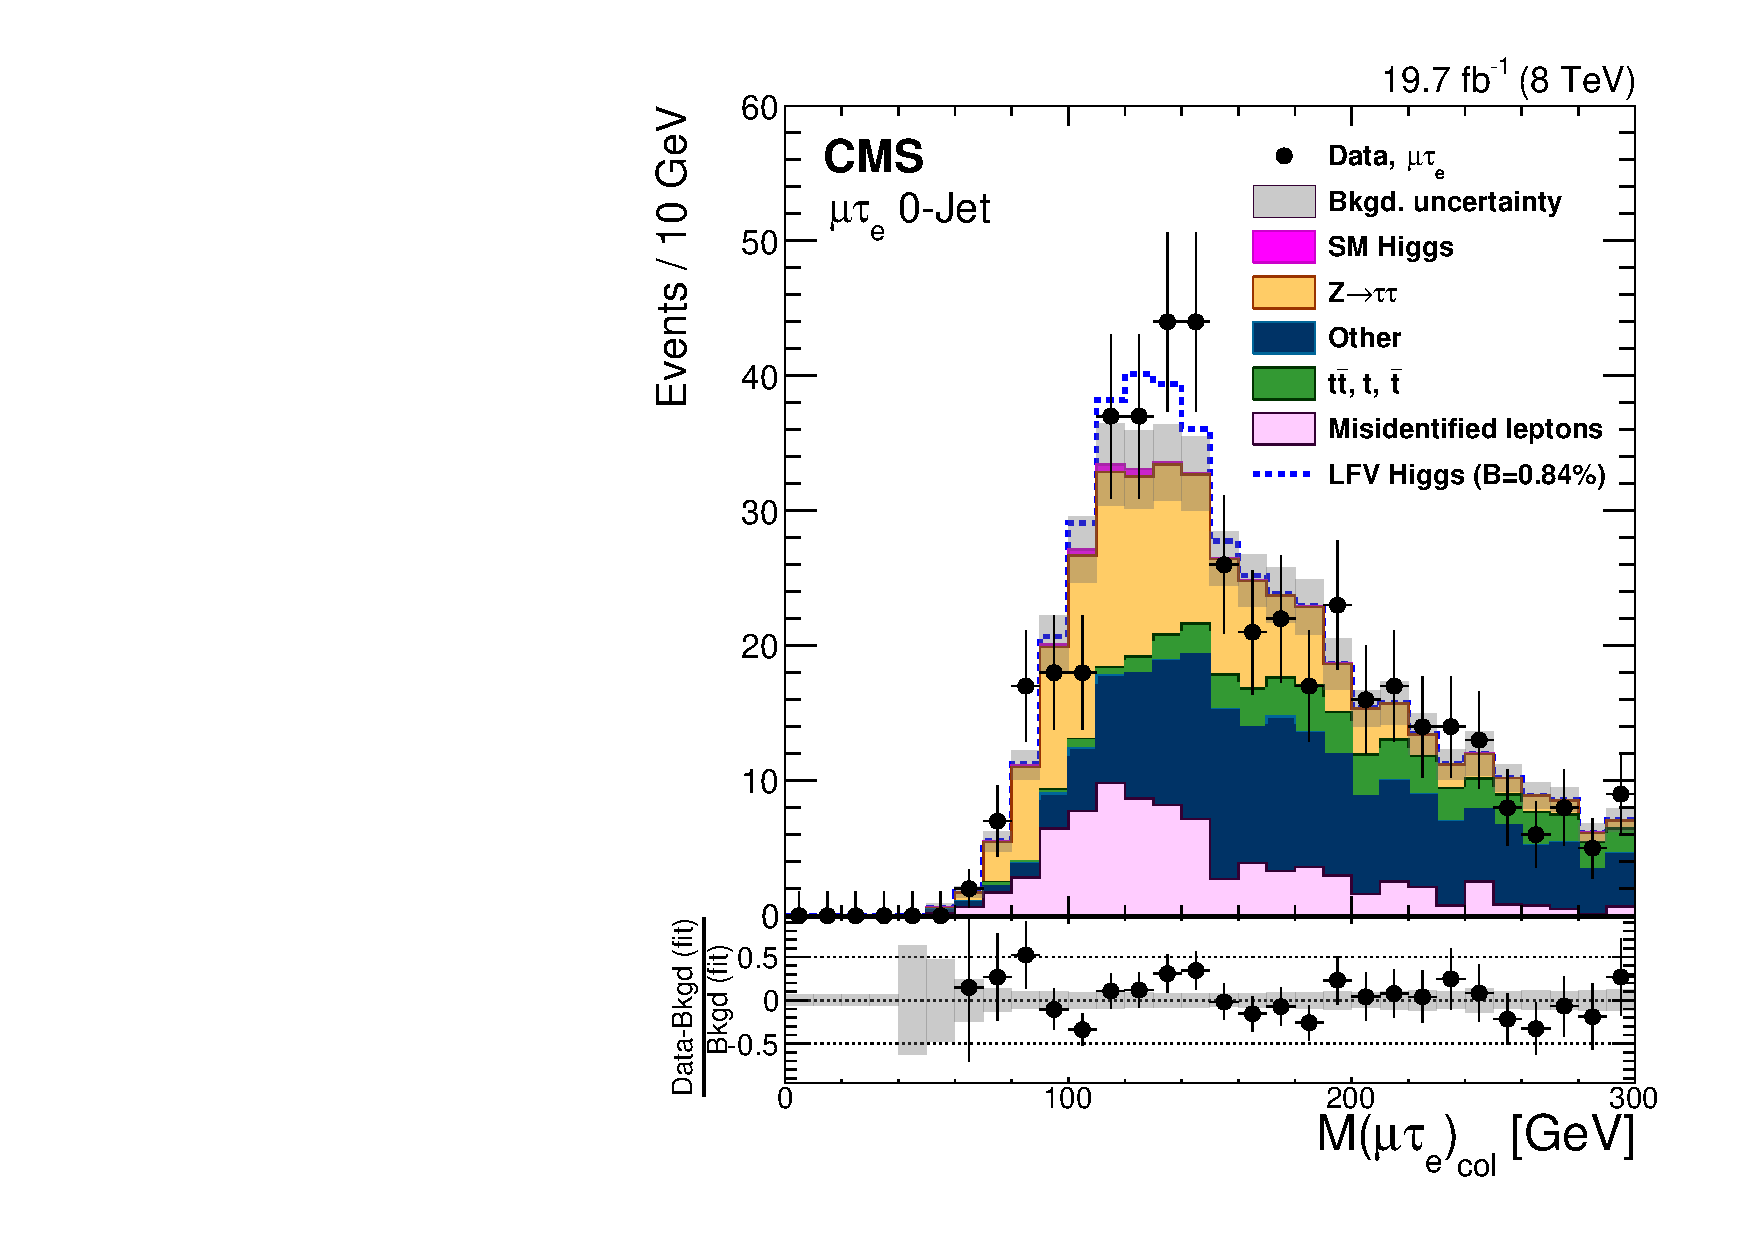
\includegraphics[width=0.48\textwidth]{muele_GG_m_colinear_UNBLIND_PostFit.pdf}
 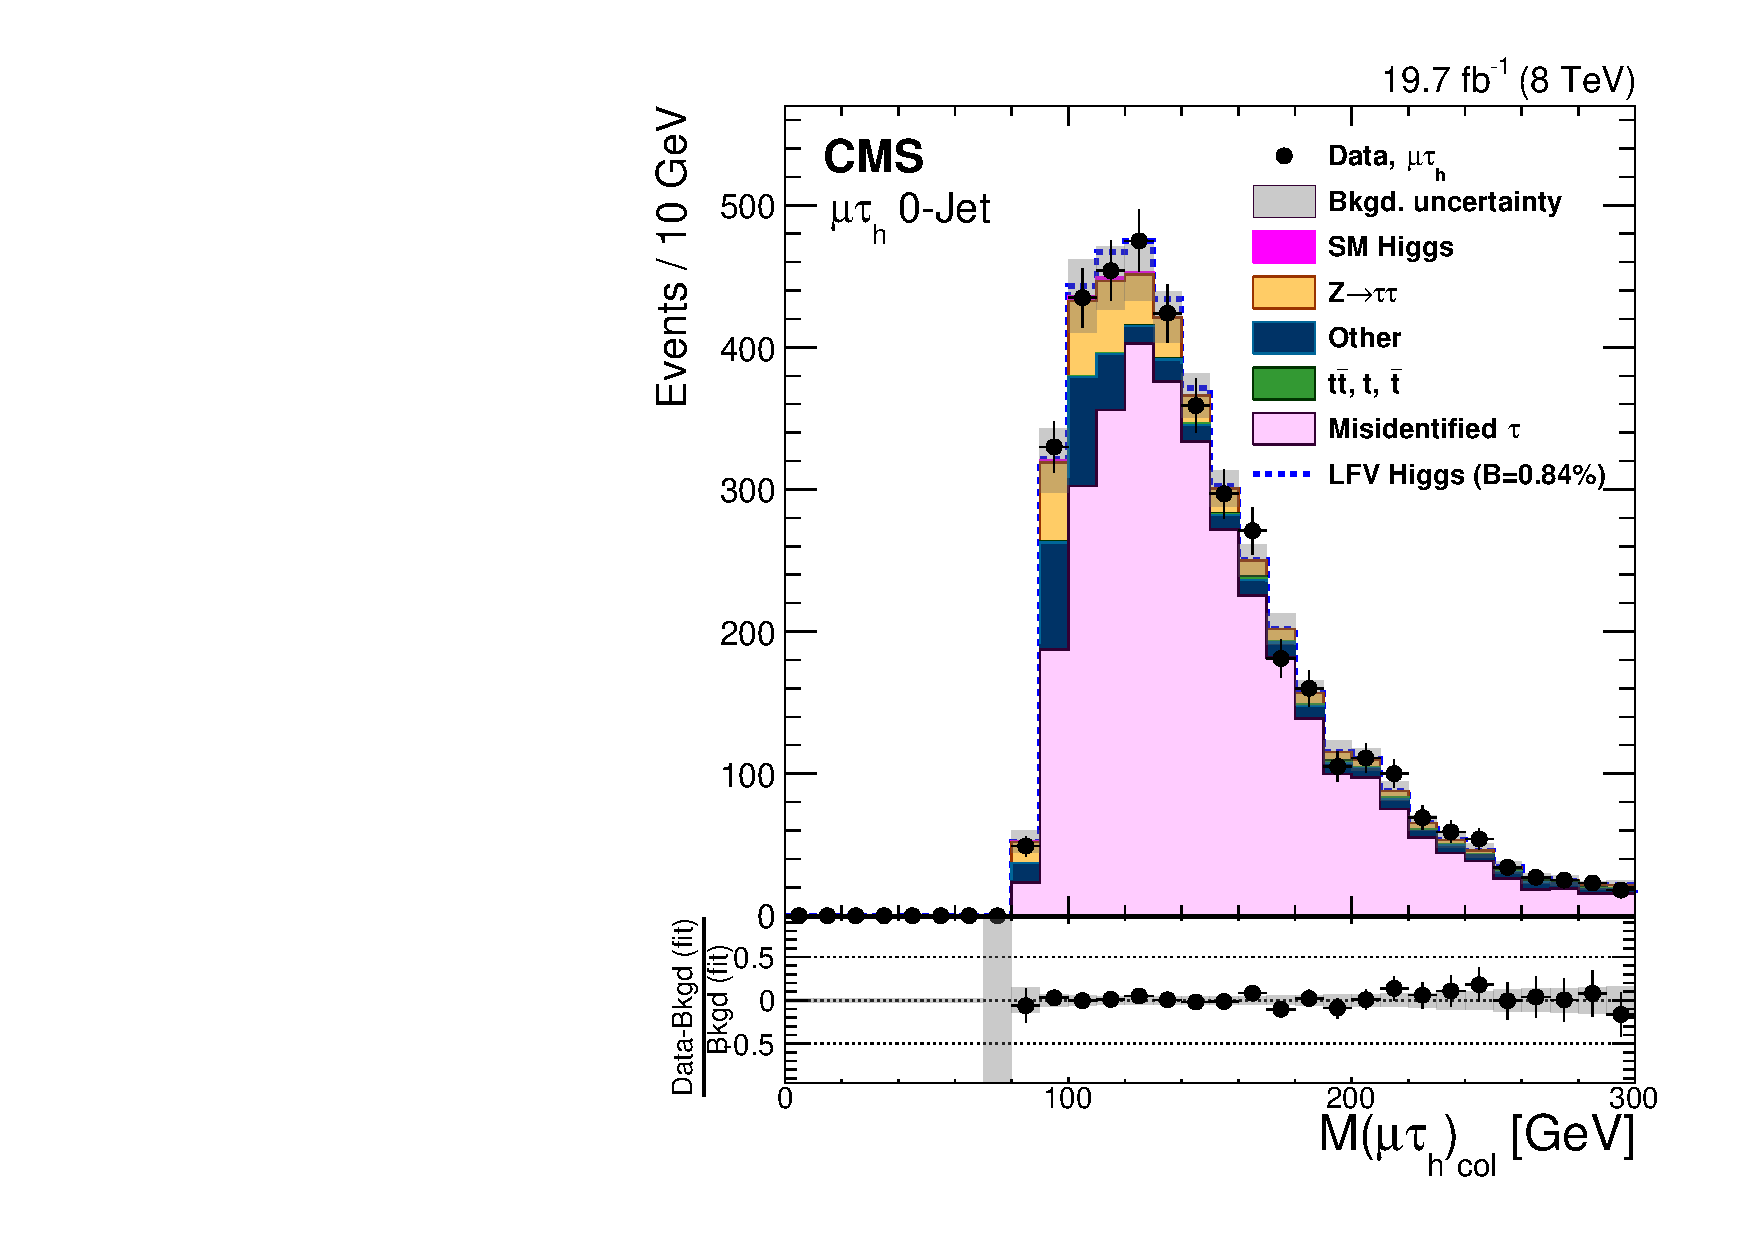
\includegraphics[width=0.48\textwidth]{muhad_GG_m_colinear_UNBLIND_PostFit.pdf}
 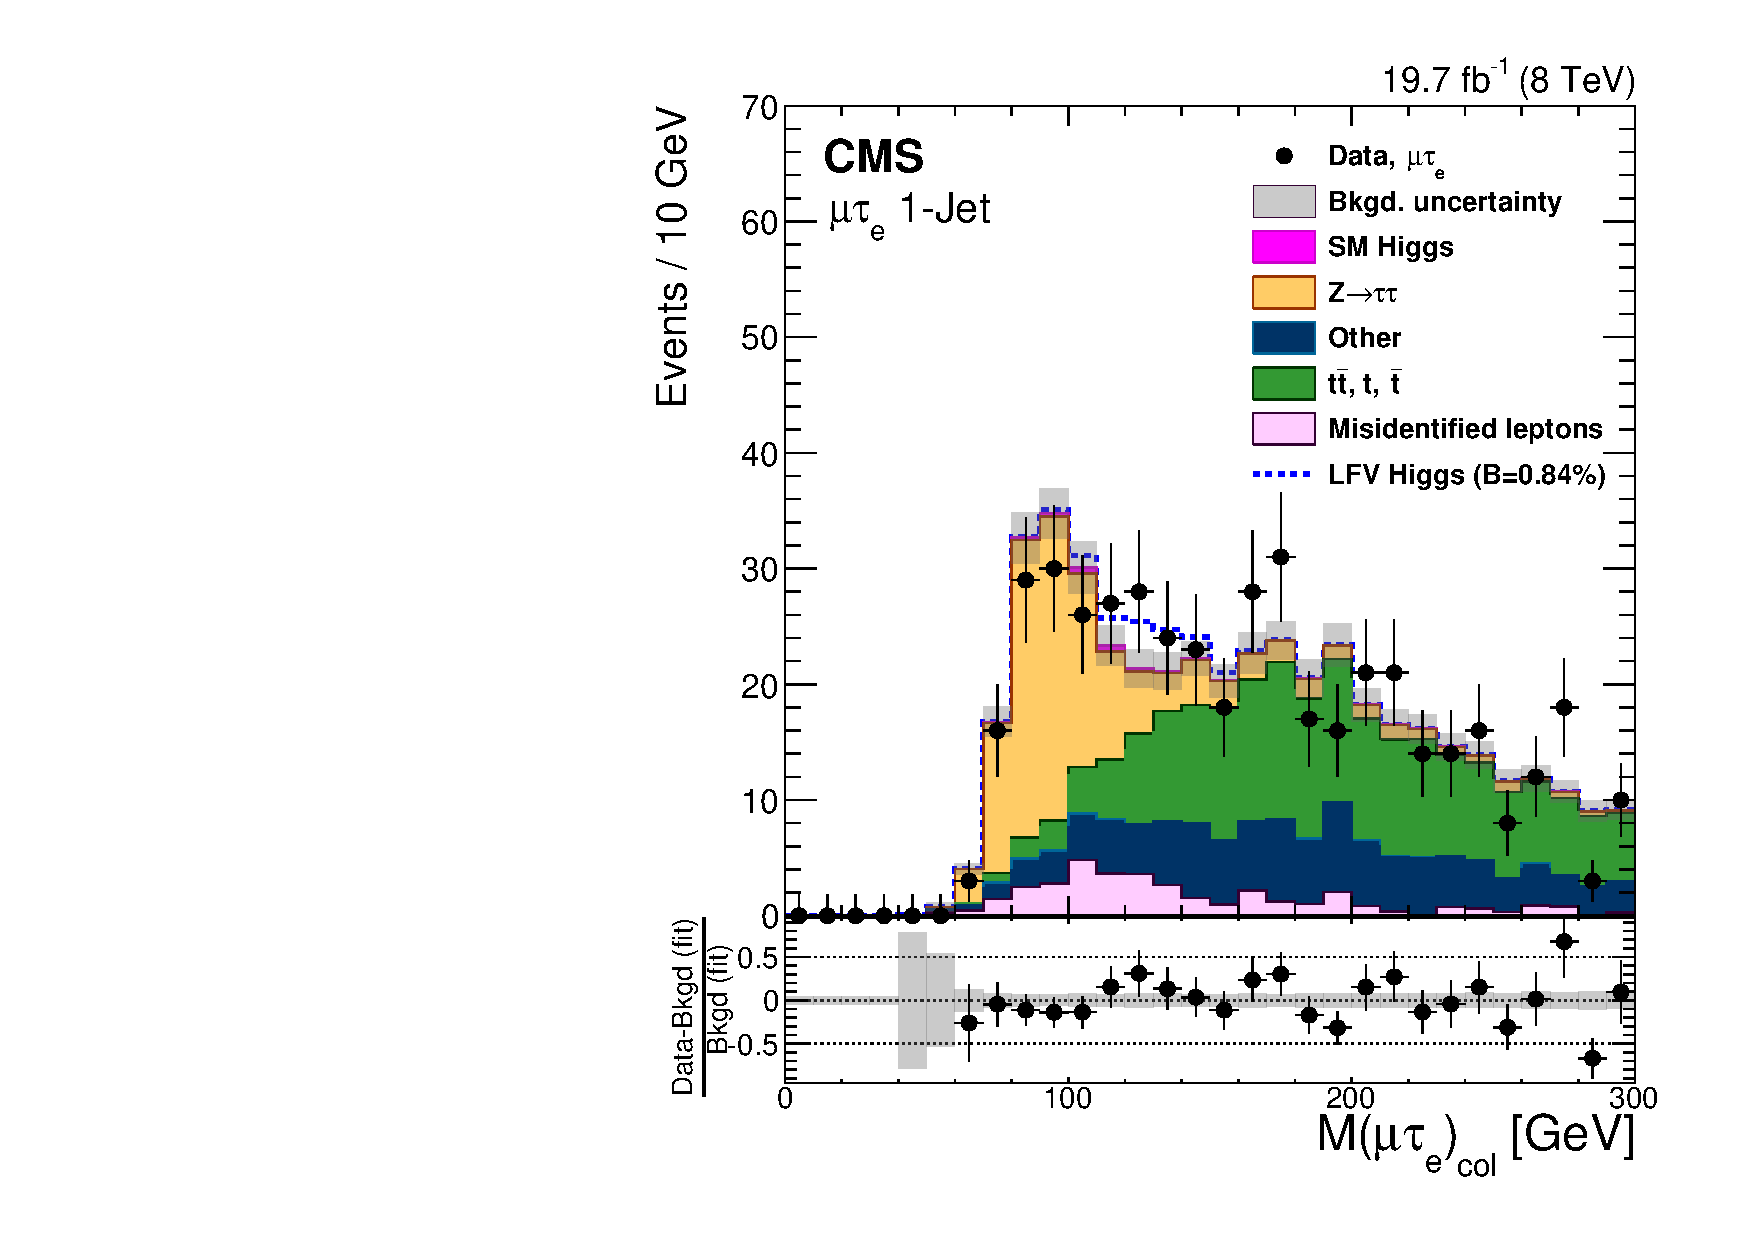
\includegraphics[width=0.48\textwidth]{muele_Boost_m_colinear_UNBLIND_PostFit.pdf}
 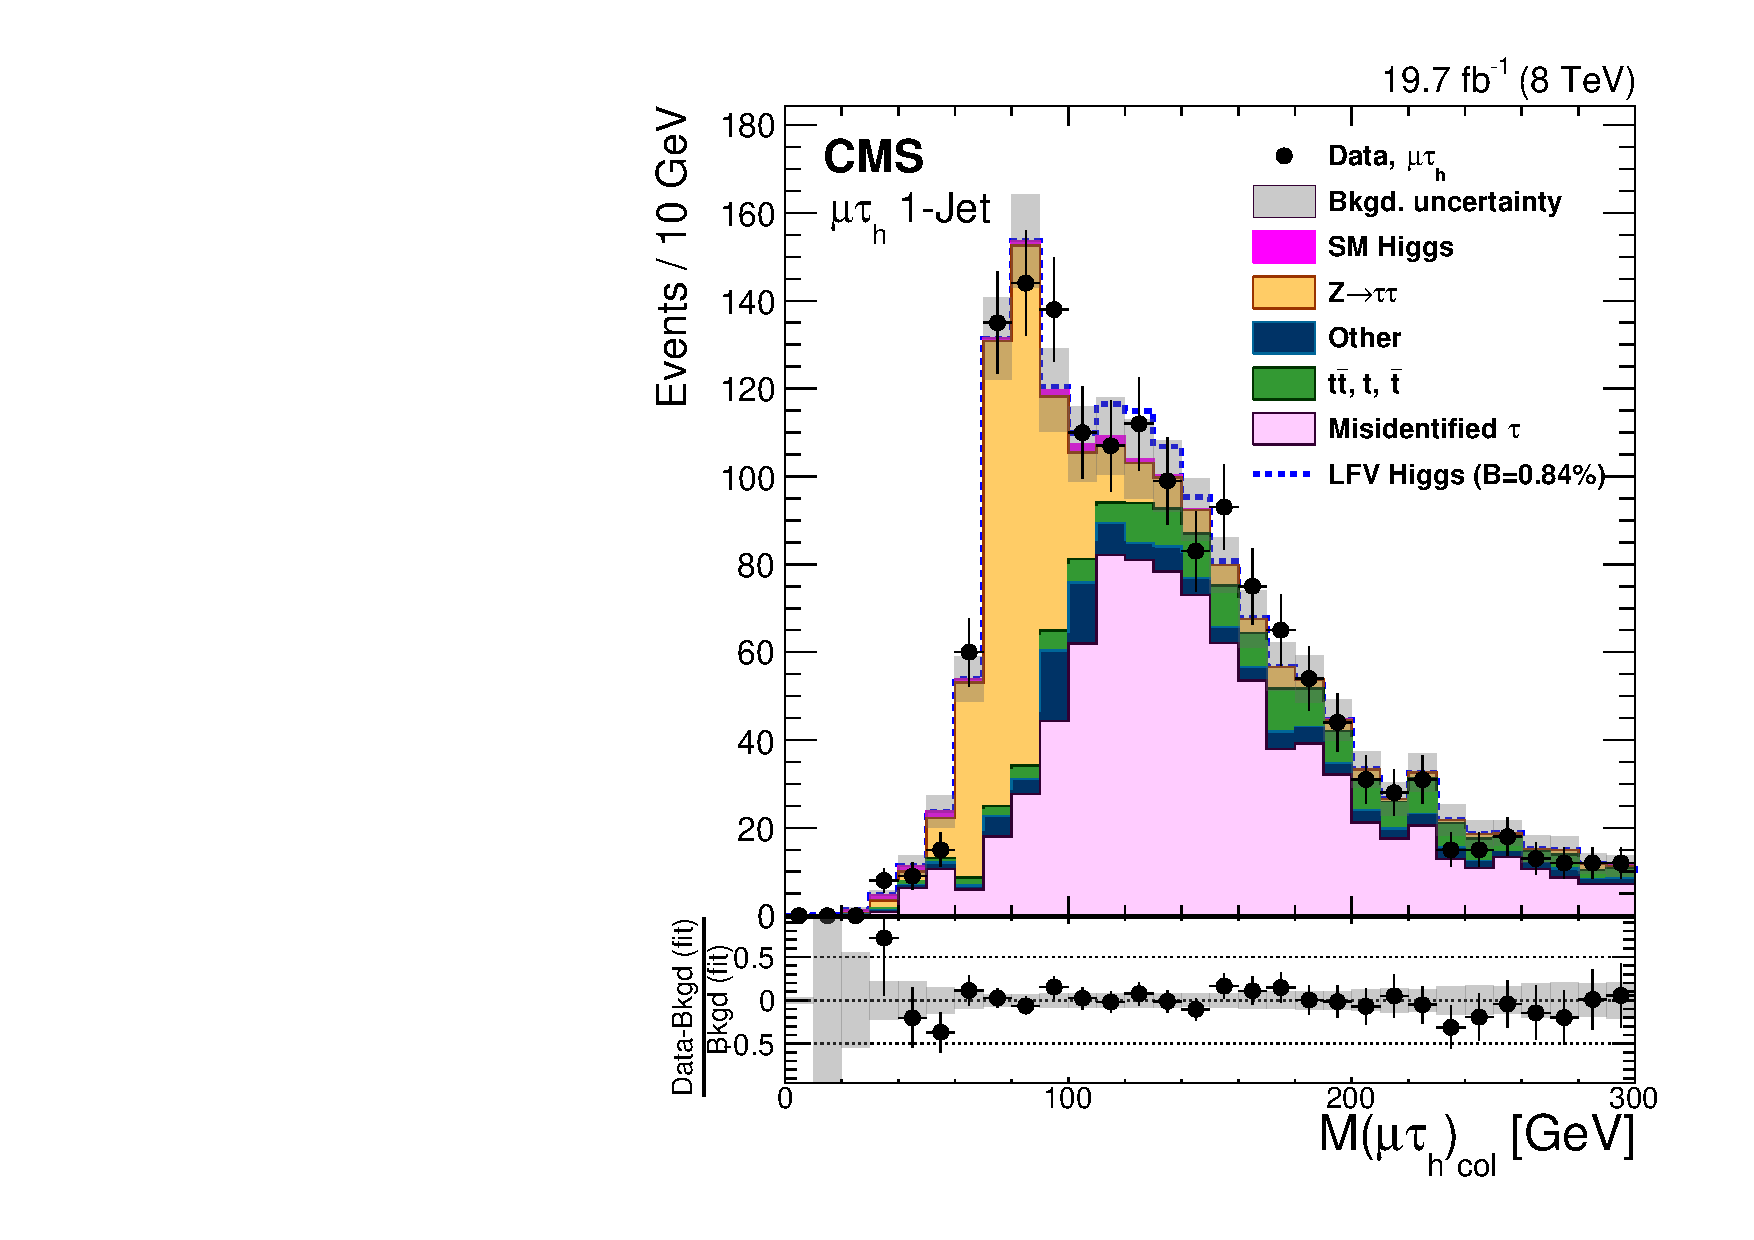
\includegraphics[width=0.48\textwidth]{muhad_Boost_m_colinear_UNBLIND_PostFit.pdf}
 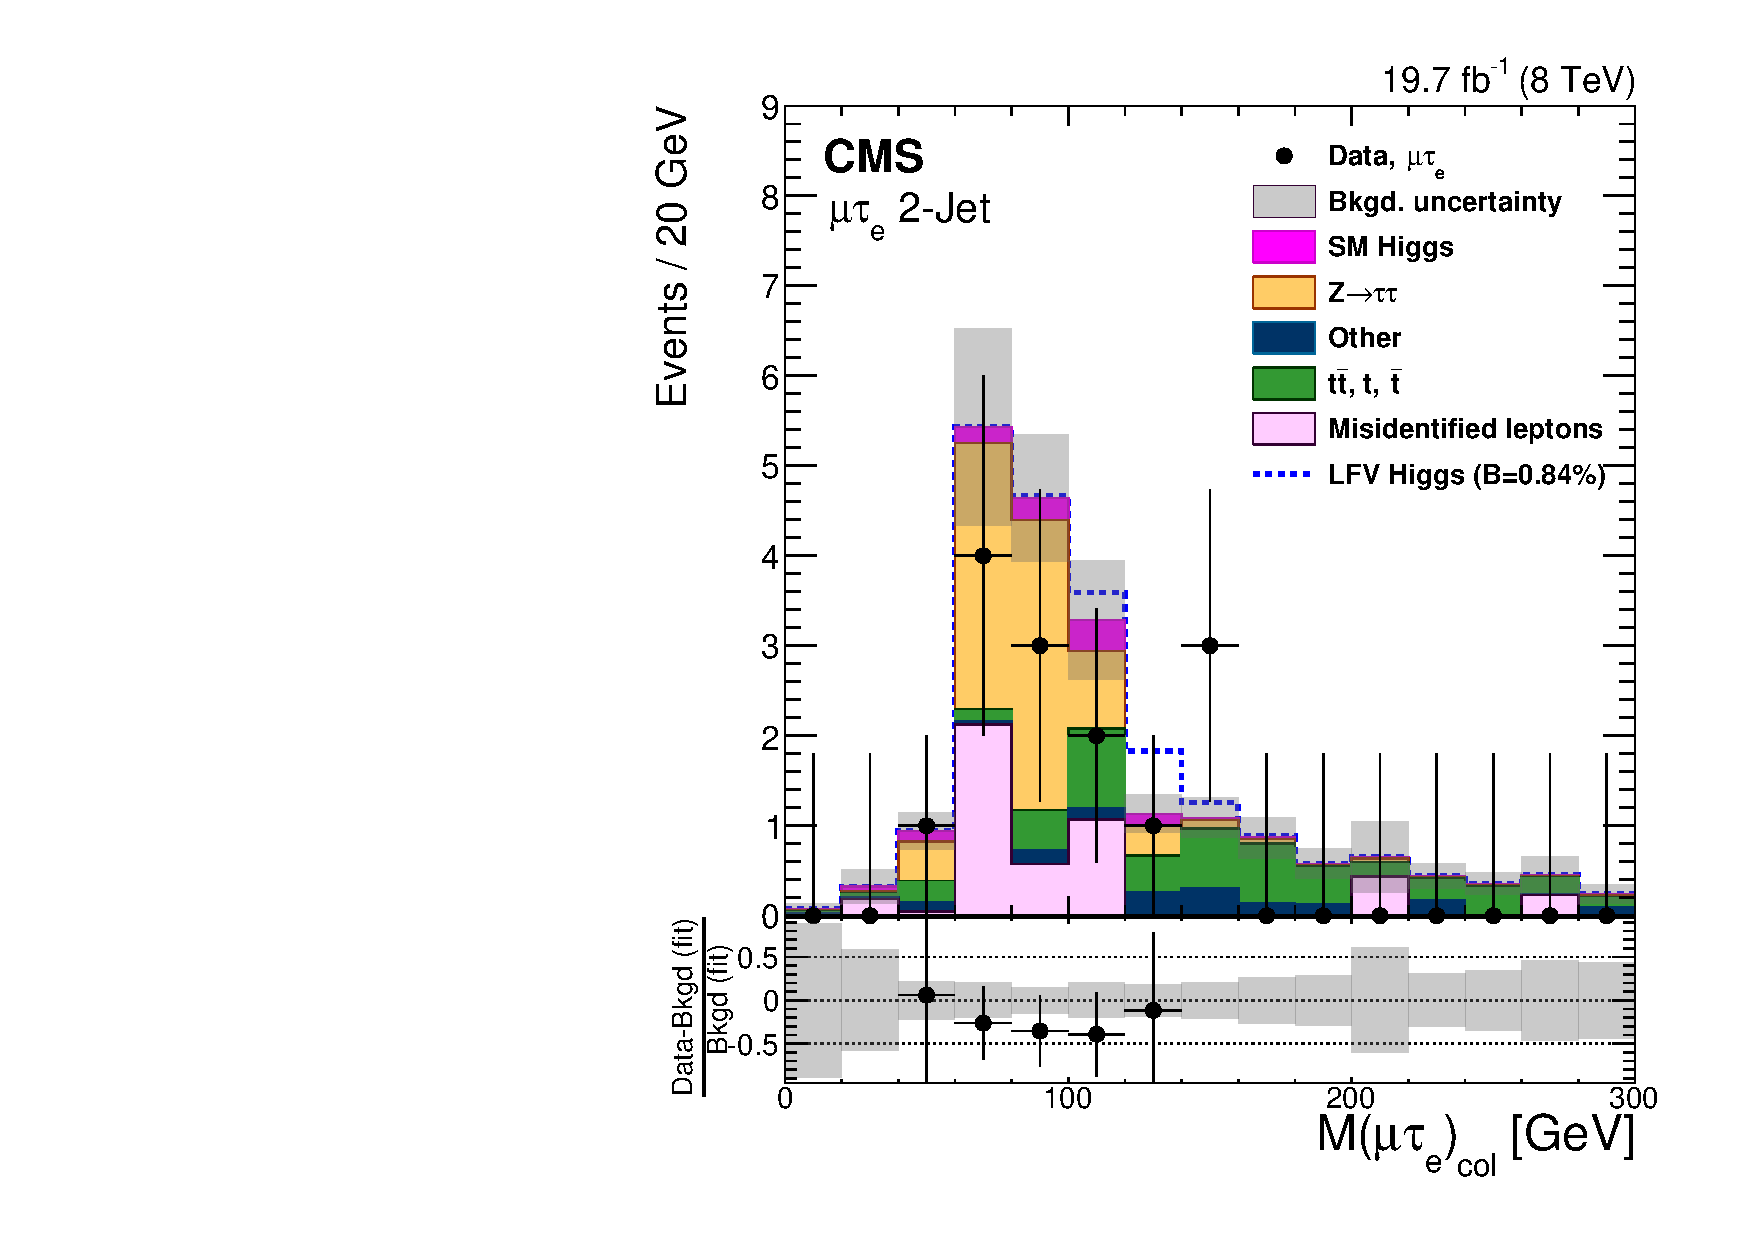
\includegraphics[width=0.48\textwidth]{muele_VBF_m_colinear_UNBLIND_PostFit.pdf}
 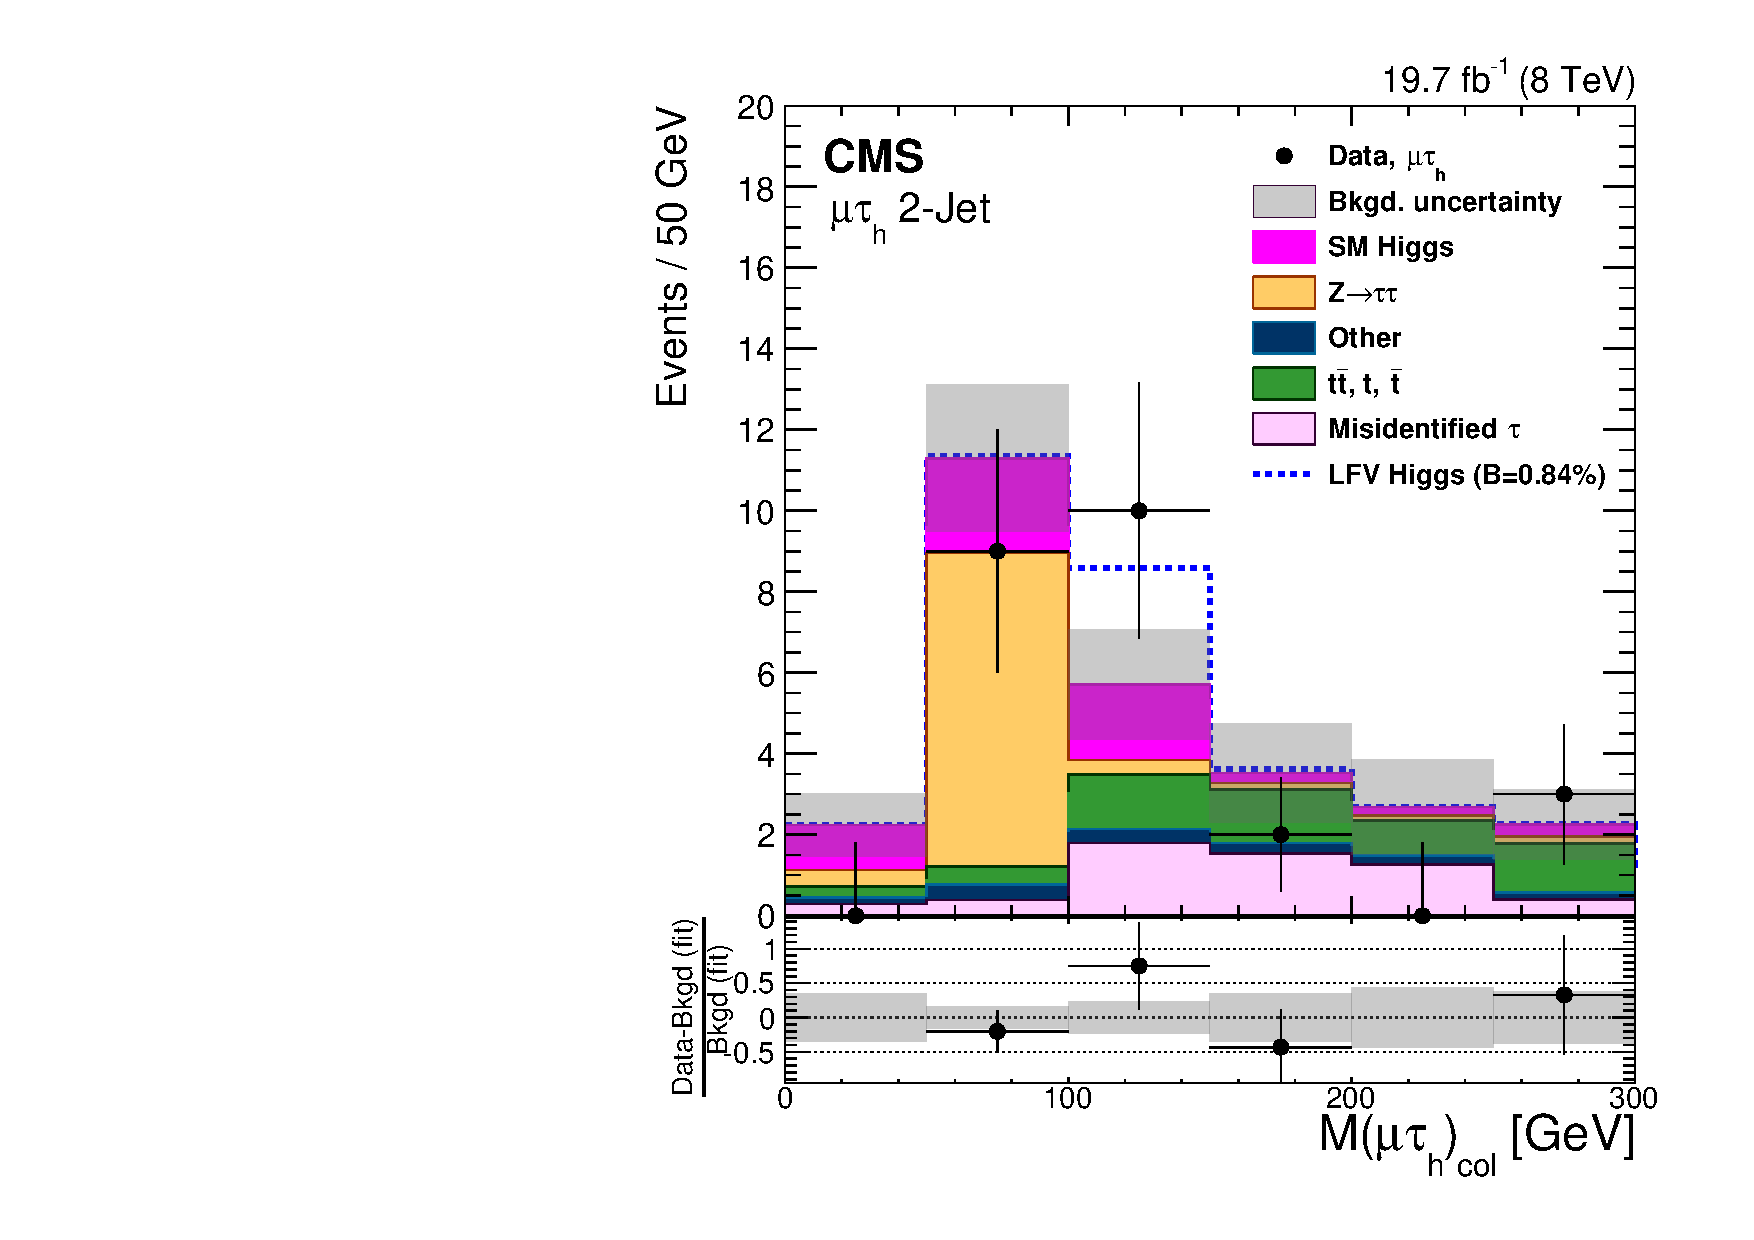
\includegraphics[width=0.48\textwidth]{muhad_VBF_m_colinear_UNBLIND_PostFit.pdf}
 \caption{Distributions of the collinear mass $M_\text{col}$ after fitting for signal and background  for the LFV $H \rightarrow \mu \tau$ candidates in
the different
channels and categories compared to data.
The distribution of the simulated LFV Higgs boson sample is shown for the best fit branching fraction
of $B(H \rightarrow \mu \tau )=0.84\%$.
The bottom panel in each plot shows the fractional difference between the observed data and the fitted background. Top left: $H \rightarrow \mu \tau_{e}$ 0-jet; top right: $H \rightarrow \mu \tau_{h}$ 0-jet;
middle left: $H \rightarrow \mu \tau_{e}$ 1-jet; middle right: $H \rightarrow \mu \tau_{h}$ 1-jet; bottom left: $H \rightarrow \mu \tau_{e}$ 2-jet; bottom right $H \rightarrow \mu \tau_{h}$ 2-jet.}
 \label{fig:Mcol_Postfit}\end{figure*}

\begin{table*}[hbtp]
 \centering
  \caption{Event yields in the signal region,  $100\: <  M_\text{col} < 150GeV $ after fitting for signal and background. The expected contributions are normalized to an integrated luminosity
of 19.7 $fb^{-1}$. The LFV Higgs boson signal is the expected yield for $B(H \rightarrow \mu \tau)=0.84\%$ with the SM Higgs boson cross section.}
  \label{tab:EventYieldTable_100_to_150}
  \begin{tabular}{lccc|ccc} \hline
        \multirow{2}{*}{Sample}                                & \multicolumn{3}{c}{$H \rightarrow \mu \tau_{h}$}                &     \multicolumn{3}{c}{$H \rightarrow \mu \tau_{e}$}     \\ \cline{2-7}
                                              &  0-Jet            & 1-Jet            & 2-Jets               &  0-Jet             & 1-Jet            & 2-Jets  \\ \hline
    misidentified leptons                          &  $  1770 \pm 530$      & $   377 \pm 114$      &  $     1.8 \pm   1.0$&  $    42 \pm  17$    &$    16 \pm   7$      & $     1.1 \pm   0.7$  \\
    $ Z \rightarrow \tau \tau$                        &  $   187 \pm   10$     & $    59 \pm   4$      &  $     0.4 \pm   0.2$&  $    65 \pm   3$    &$    39 \pm   2$      & $     1.3 \pm   0.2$   \\
    $ ZZ,WW$                                  &  $    46 \pm   8$      & $    15 \pm   3$      &  $     0.2 \pm   0.2$&  $    41 \pm   7$    &$    22 \pm   4$      & $     0.7 \pm   0.2$    \\
    $ W\gamma$                                &  NA  & NA  &  NA &  $     2 \pm   2$    &$     2 \pm   2$      & NA    \\
    $ Z \rightarrow ee$ or $\mu \mu$                  &  $   110 \pm  23$      & $    20 \pm   7$      &  $     0.1 \pm   0.1$&  $     1.6 \pm   0.7$&$     1.8 \pm   0.8$  & NA                  \\
    $t\bar{t}     $                      &  $     2.2 \pm   0.6$  & $    24 \pm   3$      &  $     0.9 \pm   0.5$&  $     4.8 \pm   0.7$&$    30 \pm   3$      & $     1.8 \pm   0.4$   \\
    $t\bar{t}   $                      &  $     2.2 \pm   1.1$  & $    13 \pm   3$      &  $     0.5 \pm   0.5$&  $     1.9 \pm   0.2$&$     6.8 \pm   0.8$  & $     0.2 \pm   0.1$   \\
    SM H background                       &  $     7.1 \pm   1.3$  & $     5.3 \pm   0.8$  &  $     1.6 \pm   0.5$&  $     1.9 \pm   0.3$&$     1.6 \pm   0.2$  & $     0.6 \pm   0.1$    \\
    sum of backgrounds                        &  $  2125 \pm 530$      & $   513 \pm 114$      &  $     5.4 \pm   1.4$&  $   160 \pm  19$    &$   118 \pm   9$     & $     5.6 \pm   0.9$    \\   \hline
    LFV Higgs boson signal                          &  $    66 \pm  18$      & $    30 \pm   8$      &  $     2.9 \pm   1.1$&  $    23 \pm   6$    &$    13 \pm   3$      & $     1.2 \pm   0.3$    \\   \hline
    data                                      &  $  2147 $             & $   511 $             &  $    10 $           &  $   180 $           &$   128 $             & $     6 $    \\   \hline
  \end{tabular}

\end{table*}

 The observed and the median expected $95\%$ $CL_{s}$ upper limits on the $B(H \rightarrow \mu \tau )$ for the H mass at 125 GeV are given for each category
 in Table~\ref{tab:expected_limits}.  Combining all
the channels, an expected upper limit of $B(H \rightarrow \mu \tau )<(0.75 \pm 0.38)\%$ is obtained. The
observed upper limit is $B(H \rightarrow \mu \tau ) < 1.51\%$ which is above the expected limit due to an excess of the
observed number of events above the background prediction.
The fit can then be used to estimate the branching fraction if this excess were to be interpreted as a signal.
The best fit values for the branching fractions are given in Table~\ref{tab:expected_limits}.
The limits and best fit branching fractions are also  summarized graphically  in
Fig.~\ref{fig:limits_summary}. The combined categories give a best fit of $B(H \rightarrow \mu \tau )=(0.84^{+0.39}_{-0.37})\%$. The combined excess is 2.4 standard deviations which corresponds to a  $p$-value of 0.010 at $M_{H}=125$ GeV.

\begin{table}[hbtp]
 \centering
  \caption{The expected upper limits, observed upper limits and best fit values for the branching fractions for different
    jet categories for the $H \rightarrow \mu \tau$  process.
    The one standard-deviation probability intervals around the expected limits are shown in parentheses.}
  \label{tab:expected_limits}
   \begin{tabular}{l|c|c|c} \hline
\multicolumn{4}{c}{Expected Limits} \\ \hline
                       &  \multicolumn{1}{c|}{0-Jet}   & \multicolumn{1}{c}{1-Jet}    &  \multicolumn{1}{|c}{2-Jets}                 \\
                       & (\%)                     & (\%)                     & (\%)                    \\ \cline{2-4}
          $\mu\tau_{e}$  &  $<$1.32 ($\pm$0.67)   &  $<$1.66 ($\pm$0.85)   &  $<$3.77 ($\pm$1.92)  \\
      $\mu\tau_{h}$    &  $<$2.34 ($\pm$1.19)   &  $<$2.07 ($\pm$1.06)   &  $<$2.31 ($\pm$1.18)  \\ \hline
            $\mu\tau$  &        \multicolumn{3}{c}{  $<$0.75 ($\pm$0.38 ) }                              \\ \hline
\multicolumn{4}{c}{Observed Limits} \\ \hline
          $\mu\tau_{e}$  &  $<$2.04                &  $<$2.38                &  $<$3.84   \\
      $\mu\tau_{h}$    &  $<$2.61                &  $<$2.22                &  $<$3.68   \\ \hline
            $\mu\tau$  & \multicolumn{3}{c}{  $<$1.51 }   \\ \hline
\multicolumn{4}{c}{Best Fit Branching Fractions} \\ \hline
      \rule[-5pt]{0pt}{17pt}
      $\mu\tau_{e}$  &  $0.87^{+0.66}_{-0.62}$  &  $0.81^{+0.85}_{-0.78}$  &  $0.05^{+1.58}_{-0.97}$  \\
      \rule[-5pt]{0pt}{17pt}
      $\mu\tau_{h}$    &  $0.41^{+1.20}_{-1.22}$  &  $0.21^{+1.03}_{-1.09}$  &  $1.48^{+1.16}_{-0.93}$  \\ \hline
      \rule[-5pt]{0pt}{17pt}
      $\mu\tau$  & \multicolumn{3}{c}{ $0.84^{+0.39}_{-0.37}$ }   \\ \hline
  \end{tabular}
\end{table}
\begin{figure*}[hbtp]\centering
\includegraphics[width=0.48\textwidth]{NewMETLimits.pdf}
 \caption{95\% CL Upper limits by category for the LFV $H \rightarrow \mu \tau$  decays}
 \label{fig:limits_summary}\end{figure*}

%\section{Limits on lepton-flavour-violating couplings}
%\begin{figure}[hbt]\centering
%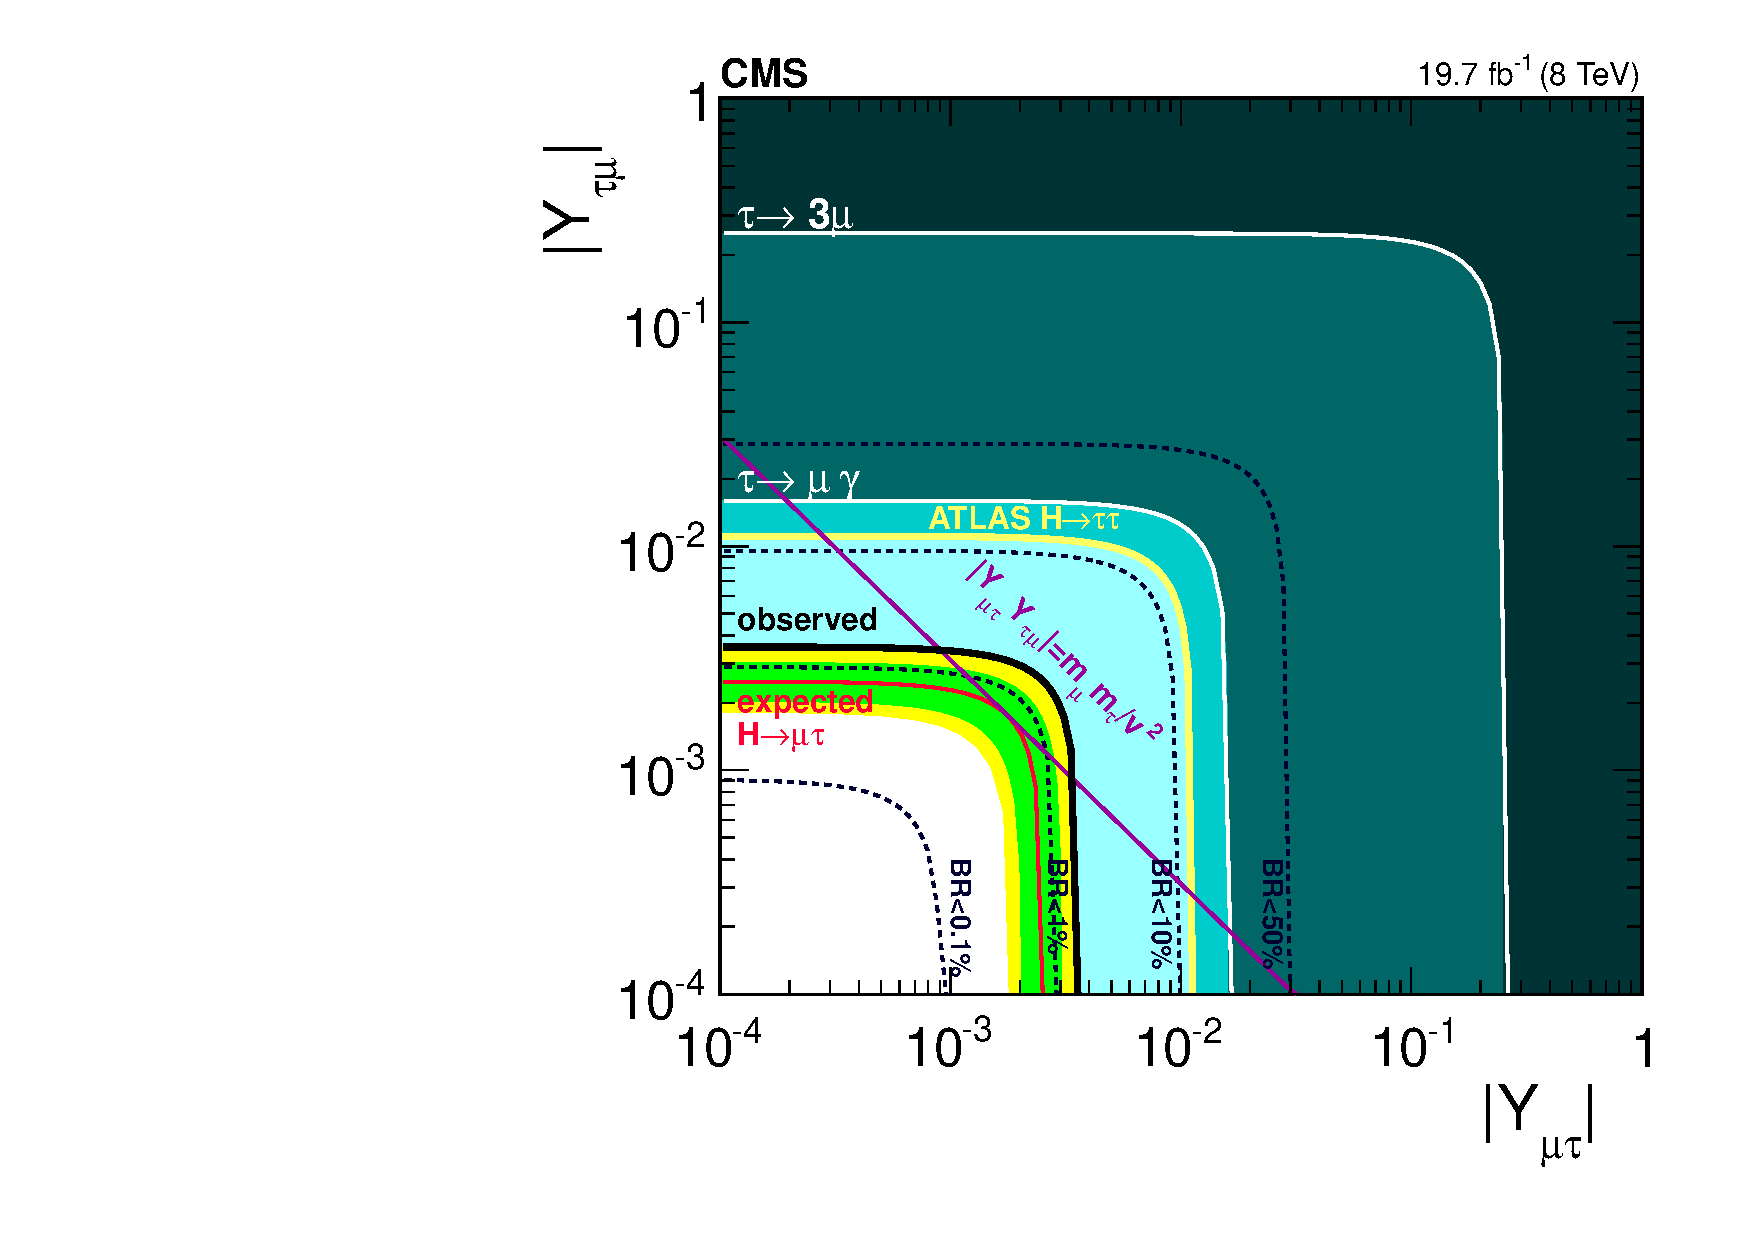
\includegraphics[width=0.49\textwidth]{yukawa.pdf}
% \caption{Constraints on the flavour-violating Yukawa couplings, $\abs{Y_{\mu\tau}}$ and $\abs{Y_{\tau\mu}}$.
%The black dashed lines are contours of $B(H \rightarrow \mu \tau )$ for reference.
%The expected limit (red solid line) with one sigma (green)  and two sigma (yellow) bands, and observed limit (black solid line) are derived from the limit on $B(H \rightarrow \mu \tau )$ from the present analysis.  The shaded regions are derived constraints from null searches for $\tau \rightarrow 3\mu$ (dark green) and $\tau \rightarrow \mu \gamma$ (lighter green). 
%The yellow line is the limit from a theoretical reinterpretation of an ATLAS $H \rightarrow \tau \tau$ search~\cite{Harnik:2012pb}.
%The light blue region indicates the additional parameter space excluded by our result.
%The purple diagonal line is the theoretical naturalness
%limit $Y_{ij}Y_{ji} \leq m_im_j/v^2$. }
% \label{fig:yukawalimits}\end{figure}

%The constraint on $B(H \rightarrow \mu \tau )$ can be interpreted in terms of LFV  Yukawa couplings~\cite{Harnik:2012pb}.
%The LFV decays $H \rightarrow e\mu$, $e\tau$, $\mu\tau$ arise at tree level from the assumed
%flavour-violating Yukawa interactions, $Y_{\ell^{\alpha}\ell^{\beta}}$ where $\ell^{\alpha},\ell^{\beta}$ denote the leptons, $\ell^{\alpha},\ell^{\beta}=e,\mu,\tau$ and $\ell^{\alpha}\neq \ell^{\beta}$.
%The decay width $\Gamma(H \rightarrow \ell^{\alpha}\ell^{\beta})$  in terms of the Yukawa couplings is given by:
%\begin{equation*}
%\Gamma(H \rightarrow \ell^{\alpha}\ell^{\beta})=\frac{m_{H}}{8\pi}\bigl(\abs{Y_{\ell^{\beta}\ell^{\alpha}}}^2 + \abs{Y_{\ell^{\alpha}\ell^{\beta}}}^2\bigr),
%\end{equation*}
%and the branching fraction by:
%\begin{equation*}
%B(H \rightarrow \ell^{\alpha}\ell^{\beta})=\frac{\Gamma(H\rightarrow \ell^{\alpha}\ell^{\beta})}{\Gamma(H\rightarrow \ell^{\alpha}\ell^{\beta}) + \Gamma_{SM}}.
%\end{equation*}
%The SM H decay width is assumed to be $\Gamma_{\mathrm{SM}}=4.1$MeV~\cite{Denner:2011mq} for $M_{H}=125GeV$.
%The 95\% CL constraint on the Yukawa couplings derived from $B(H \rightarrow \mu \tau )<1.51\%$ and the expression for the branching fraction above is:\begin{equation*}
%\sqrt{\abs{Y_{\mu\tau}}^{2}+\abs{Y_{\tau\mu}}^{2}}<3.6\times 10^{-3}.
%\end{equation*}
%Figure~\ref{fig:yukawalimits} compares this result to the constraints from previous indirect
%measurements.


\subsection{13 TeV Results}
After applying the full selection cuts, a maximum likelihood fit is performed in the $M_\text{col}$ variable. Each systematic uncertainty is used as a nuisance parameter in the fit. The distributions of the signal and background contributions after the full selection and the fit are shown in Fig.~\ref{fig:Mcol_SignalRegion} and the
event yields in the mass range $100\:  < M_\text{col} < 150GeV$ are shown in Table~\ref{tab:EventYieldTable_100_to_150}.
The different channels and categories are combined  to set a $95\%$ CL  upper limit on the branching
fraction of LFV H decay in the  $\mu\Pgt$ channel, $\mathcal{B}(H\rightarrow\mu\Pgt)$.

\begin{figure*}[hbtp]\centering
% \includegraphics[width=0.48\textwidth]{Plots/HMuE/SignalOS/LFVMuE_SR_OS_0Jet_UnBlinded_Postfit.pdf}
% \includegraphics[width=0.48\textwidth]{Plots/HMuTau/SignalOS/LFVMuTau_SR_OS_0Jet_UnBlinded_Postfit.pdf}
% \includegraphics[width=0.48\textwidth]{Plots/HMuE/SignalOS/LFVMuE_SR_OS_1Jet_UnBlinded_Postfit.pdf}
% \includegraphics[width=0.48\textwidth]{Plots/HMuTau/SignalOS/LFVMuTau_SR_OS_1Jet_UnBlinded_Postfit.pdf}
% \includegraphics[width=0.48\textwidth]{Plots/HMuE/SignalOS/LFVMuE_SR_OS_2Jet_UnBlinded_Postfit.pdf}
% \includegraphics[width=0.48\textwidth]{Plots/HMuTau/SignalOS/LFVMuTau_SR_OS_2Jet_UnBlinded_Postfit.pdf}
\caption{Distributions of the collinear mass $M_\text{col}$ after fitting for signal and background  for the LFV $H \rightarrow \mu \Pgt$ candidates in
the different
channels and categories compared to data.
The distribution of the simulated LFV Higgs boson sample is shown for $\mathcal{B}(H \rightarrow \mu \Pgt )=10\%$.
The bottom panel in each plot shows the fractional difference between the observed data and the fitted background. Top left: $H \rightarrow \mu \Pgt_{e}$ 0-jet; top right: $H \rightarrow \mu \tauh$ 0-jet;
middle left: $H \rightarrow \mu \Pgt_{e}$ 1-jet; middle right: $H \rightarrow \mu \tauh$ 1-jet; bottom left: $H \rightarrow \mu \Pgt_{e}$ 2-jet;
bottom right $H \rightarrow \mu \tauh$ 2-jet.}
 \label{fig:Mcol_SignalRegion}\end{figure*}
 
 \begin{table*}[hbtp]
 \centering  \caption{Event yields in the signal region in the range $100 < M_\text{col} < 150GeV$ . The expected contributions are normalized to an integrated luminosity
of 2.3$fb^{-1}$. The LFV Higgs boson signal is the expected yield for $B(H \rightarrow \mu \tau)=1\%$ with the SM Higgs boson cross section.}
  \label{tab:EventYieldTable_100_to_150}
%   \cmsTable{\textwidth}{
  \begin{tabular}{lccc|ccc} \hline
        \multirow{2}{*}{Sample}                                & \multicolumn{3}{c}{$H \rightarrow \mu \Pgt_{e}$}                &     \multicolumn{3}{c}{$H \rightarrow \mu \tauh$}     \\ \cline{2-7}
                                              &  0-Jet            & 1-Jet            & 2-Jets               &  0-Jet             & 1-Jet            & 2-Jets  \\ \hline
    misidentified leptons                    &  12.2  &   5.2     &  2.8 & 232.3 & 54.7 & 4.7 \\
    $ \cPZ \rightarrow \Pgt \Pgt$                    & 14.4   & 10.6      &  1.7 & 5.3   & 2.3  & 0  \\
    $ \cPZ\cPZ,WW$                       & 10.7   &  4.6      &  3.2 & 3.2   & 2.0  & 0.3\\
    $ W\gamma$                             &   1.2  &  3.4      &  0.9 &NA & NA & NA    \\
    $ \cPZ \rightarrow ee$ or $\mu \mu$          &  1.9   &  2.2      &  0.3 & 79.1 & 11.9& 0.1  \\
    $t\bar{t}     $                            &  1.4   & 21.8      & 18.6 &1.3 & 5.4 & 1.1    \\
    t, $\bar{t}$                             &  0.4   &  4.1      &  1.7 &0.3 & 2.2 & 0.2    \\
    SM H background                        &  0.4   &  0.4      &  0.4 &1.1 & 0.7 & 0.3    \\ \hline
    sum of backgrounds                       & 42.6   & 52.2      & 29.6 &322.5& 79.3 & 6.6  \\  \hline
    LFV Higgs boson signal                   &  7.1   &  3.7      &  1.9 &13.8 & 4.7 & 1.2    \\ \hline \hline
      Observed data                          &  33    &  41       &  31  & 315 & 77 & 7 \\ \hline
  \end{tabular}
%  }
\end{table*}


\subsection{Limit computation}

The observed and median expected $95\%$ CL upper limits on the $\mathcal{B}(H \rightarrow \mu \Pgt )$ for the H mass at 125GeV are given for each category
in Table~\ref{tab:expected_limits}.  Combining all
the channels, an expected upper limit of $\mathcal{B}(H \rightarrow \mu \Pgt )<(1.62 \pm 0.58)\%$ is obtained.
The observed upper limit is $\mathcal{B}(H \rightarrow \mu \Pgt ) < 1.20\%$.
The limits are also  summarized graphically  in
Fig.~\ref{fig:limits_summary}.

This observed limit on the branching ratio is slightly tighter than the $\mathcal{B}(H \rightarrow \mu \Pgt )<(1.51 \pm 0.83)\%$ limit obtained using the 19.7 $\textrm{fb}^{-1}$ data sample at 8 TeV analyzed in~\cite{Khachatryan:2015kon}.

\begin{table}[hbtp]
 \centering
  \caption{The observed and expected upper limits for different
    jet categories for the $H \rightarrow \mu \Pgt$  process.
    The one standard deviation probability intervals around the expected limits are shown in parentheses.}
 \label{tab:expected_limits}
\begin{tabular}{c|c|c|c|c} \hline
\multicolumn{5}{c}{Expected limits} \\ \hline
                       &  \multicolumn{1}{c|}{0-jet}   & \multicolumn{1}{c|}{1-jet}    &  \multicolumn{1}{c|}{2-jets} & \multicolumn{1}{c}{Combined}                 \\
                       & (\%)                     & (\%)                     & (\%)  &    (\%)                  \\   \cline{2-5}
          $\mu\tau_{h}$  & $<$4.17  & $<$4.89   & $<$6.41   &   $<$2.98   \\
      $\mu\tau_{\textrm{e}}$           & $<$2.24   &  $<$4.36  &  $<$7.31  &  $<$1.96    \\ \hline
            $\mu\tau$      &        \multicolumn{4}{c}{  $<$1.62  \% }                              \\ \hline \hline
\multicolumn{5}{c}{Observed limits} \\ \hline
                       &  \multicolumn{1}{c|}{0-jet}   & \multicolumn{1}{c|}{1-jet}    &  \multicolumn{1}{c|}{2-jets} & \multicolumn{1}{c}{Combined}                 \\
                       & (\%)                     & (\%)                     & (\%)  &    (\%)                  \\   \cline{2-5}
          $\mu\tau_{h}$  & $<$4.24  & $<$6.35   & $<$7.71   &   $<$3.81   \\
      $\mu\tau_{\textrm{e}}$           & $<$1.33   &  $<$3.04  &  $<$8.99  &  $<$1.15    \\ \hline
            $\mu\Pgt$      &        \multicolumn{4}{c}{  $<$1.20  \% }                              \\ \hline \hline
\multicolumn{5}{c}{Best fit branching fractions} \\ \hline
                       &  \multicolumn{1}{c|}{0-jet}   & \multicolumn{1}{c|}{1-jet}    &  \multicolumn{1}{c|}{2-jets} & \multicolumn{1}{c}{Combined}                 \\
                       & (\%)                     & (\%)                     & (\%)  &    (\%)                  \\   \cline{2-5}
      \rule[-5pt]{0pt}{17pt}
      $\mu\Pgt_{h}$  &  $0.12^{+2.02}_{-1.91}$  &  $1.70^{+2.41}_{-2.52}$  &  $1.54^{+3.12}_{-2.71}$  &   $1.12^{+1.45}_{-1.40}$   \\
      \rule[-5pt]{0pt}{17pt}
      $\mu\tau_{\textrm{e}}$    &  $-2.11^{+1.30}_{-1.89}$  &  $-2.18^{+1.99}_{-2.05}$  &  $2.04^{+2.96}_{-3.31}$ & $-1.81_{-1.32}^{+1.07}$  \\ \hline
      \rule[-5pt]{0pt}{17pt}
      $\mu\Pgt$  & \multicolumn{4}{c}{ $-0.76^{+0.81}_{-0.84}$\% }   \\ \hline
  \end{tabular}
\end{table}


\begin{figure*}[hbtp]\centering
%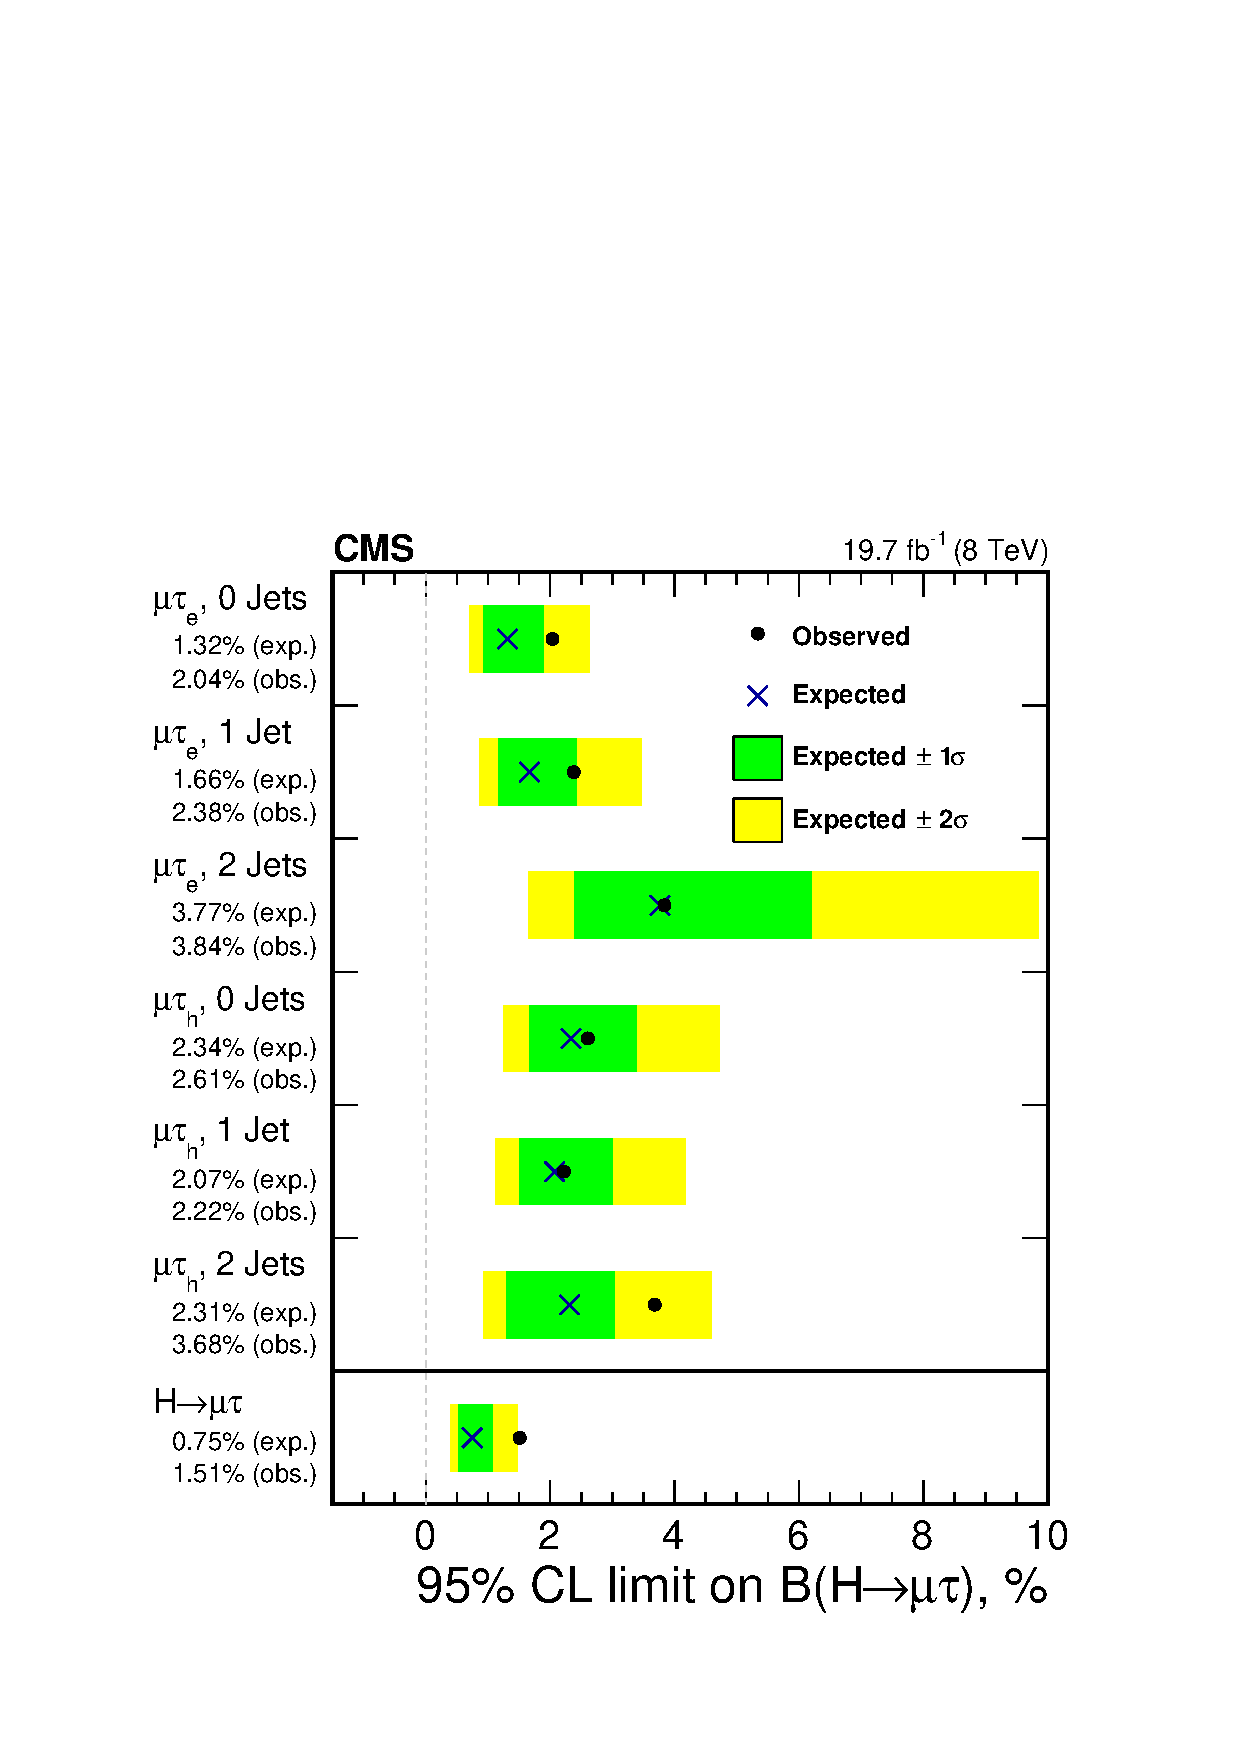
\includegraphics[width=0.48\textwidth]{Plots/Summary/plotLimit.pdf}
 \caption{95\% CL Upper limits by category for the LFV $H \rightarrow \mu \Pgt$  decays.}
 \label{fig:limits_summary}\end{figure*}

\section{Limits on lepton flavour violating couplings}
\begin{figure}[hbt]\centering
%\includegraphics[width=0.49\textwidth]{Plots/Summary/yukawa_13TeV.pdf}
 \caption{Constraints on the flavour violating Yukawa couplings, $\abs{Y_{\mu\Pgt}}$ and $\abs{Y_{\Pgt\mu}}$.
The black dashed lines are contours of $\mathcal{B}(H \rightarrow \mu \Pgt )$ for reference.
The expected limit (red solid line) with one sigma (green)  and two sigma (yellow) bands, and observed limit (black solid line) are derived from the limit on $\mathcal{B}(H \rightarrow \mu \Pgt )$ from the present analysis.  The shaded regions are derived constraints from null searches for $\Pgt \rightarrow 3\mu$ (dark green) and $\Pgt \rightarrow \mu \gamma$ (lighter green).
The light blue region indicates the additional parameter space excluded by our result.
The purple diagonal line is the theoretical naturalness
limit $Y_{ij}Y_{ji} \leq m_im_j/v^2$. }
 \label{fig:yukawalimits}\end{figure}



The constraint on $\mathcal{B}(H \rightarrow \mu \Pgt )$ can be interpreted in terms of LFV  Yukawa couplings~\cite{Harnik:2012pb}.
The LFV decays $H \rightarrow e\mu$, $e\Pgt$, $\mu\Pgt$ arise at tree level from the assumed
flavour violating Yukawa interactions, $Y_{\ell^{\alpha}\ell^{\beta}}$ where $\ell^{\alpha},\ell^{\beta}$ denote the leptons, $\ell^{\alpha},\ell^{\beta}=e,\mu,\Pgt$ and $\ell^{\alpha}\neq \ell^{\beta}$.
The decay width $\Gamma(H \rightarrow \ell^{\alpha}\ell^{\beta})$  in terms of the Yukawa couplings is given by:
\begin{equation*}
\Gamma(H \rightarrow \ell^{\alpha}\ell^{\beta})=\frac{m_{H}}{8\pi}\bigl(\abs{Y_{\ell^{\beta}\ell^{\alpha}}}^2 + \abs{Y_{\ell^{\alpha}\ell^{\beta}}}^2\bigr),
\end{equation*}
and the branching fraction by:
\begin{equation*}
B(H \rightarrow \ell^{\alpha}\ell^{\beta})=\frac{\Gamma(H\rightarrow \ell^{\alpha}\ell^{\beta})}{\Gamma(H\rightarrow \ell^{\alpha}\ell^{\beta}) + \Gamma_{SM}}.
\end{equation*}
The SM H decay width is assumed to be $\Gamma_{\mathrm{SM}}=4.1$MeV~\cite{Denner:2011mq} for $M_{H}=125GeV$.
The 95\% CL constraint on the Yukawa couplings derived from $\mathcal{B}(H \rightarrow \mu \Pgt )<1.20\%$ and the expression for the branching fraction above is:\begin{equation*}
\sqrt{\abs{Y_{\mu\Pgt}}^{2}+\abs{Y_{\Pgt\mu}}^{2}}<3.16\times 10^{-3}.
\end{equation*}
Figure~\ref{fig:yukawalimits} compares this result to the constraints from previous indirect
measurements.

\section{W+Jets}
\subsection{Detector Unfolding}
\qquad The CMS detector, like any experimental instrument, is not infallible. The detector response can cause a measurement to deviate from its true value. For example, for a given event with a leading jet $p_{T}$ in the 40-45 GeV bin, there is a probability that the jet could have had a $p_{T}$ in the 35-40 GeV bin or in the 45-50 GeV bin. The detector response can cause the measured value to deviate from its true value. A response matrix is used to transform the measured values to the true values. 

\qquad A Bayesian unfolding method~\cite{D'Agostini199548} is used for W+Jets. The $i^{th}$ generated event $Gen_{i}$ results in a measured event $Reco_{i}$. The probability of a generated event to be observed in the $i^{th}$ bin is $P(Gen_{i})$. The probability that a reco event in bin $j$ is due to a generated event in bin $i$ is $P(Reco|Gen_{i})$. From those relations, Bayes' theorem~\cite{BevingtonRobinson200207} is used to obtain $P(Gen_{i}|Reco_{j}) = \frac{P(Reco_{j}|Gen_{i})P(Gen_{i})}{\Sigma_{l=1}^{n_{bins}}P(Reco_{j}|Gen_{l})P(Gen_{l})}$

\qquad The probability to observe a reconstructed event in bin $j$ given an generator level event in bin $i$ is given by $P(Reco_{j}|Gen_{i})$. This probability is represented by a matrix, defined as the response matrix ($R_{ji}$). The response matrix is calculated by using Monte Carlo (Section 4) to compare generator level events to events reconstructed with detector simulation. It can be visualized for a particular variable by plotting the number of generator level events versus the number of reco level events. After calculating the response matrix, Bayes' theorem is used to obtain the probability that a reconstructed event in bin $j$ was due to a generator level event in bin $i$. This probability distribution, $P(Gen_{i}|Reco_{j})$, is referred to as the smearing matrix, $S_{ij}$.

\qquad The number of true events observed in bin $i$ is defined as $\hat{n}(i) = \frac{1}{\epsilon_{i}}\Sigma_{j=1}^{n_{bins}}n_{obs}(j)S_{ij}$, where $\epsilon_{i}$ is the efficiency of observing an event that was generated in bin $i$ and is defined by $\epsilon_{i}=\Sigma_{j=1}^{n_bins}R_{ji}$.

\qquad Given the above formulas, the number of true events in each bin can be calculated. The only unknown quantity is $P(Gen_{i})$, the probability to observe a generator level event in bin $i$. This probability is determined by an iterative $\chi^2$ fit. First, $P(Gen_{i})$ is estimated from the Monte Carlo distribution. This allows a simple estimation of the true number of events: $\hat{n}_{0} = P(Gen_{i})N_{obs}$, where $N_{obs}$ is the total number of observed events. Then use Bayes' Theorem to calculate $\hat{n}(i)$ and $\hat{P}(Gen_{i})$. The third step is to calculate the $\chi^{2}$ distribution between $\hat{n}(i)$ and $\hat{n}_{0}(i)$. The iterative procedure is then repeated, with $\hat{n}(i)$ and $\hat{P}(Gen_{i})$ used in the first step. The iterative procedure is repeated at least four times and is concluded when $\chi^{2}/\nu < \frac{1}{\sqrt{2}}$.

\subsection{13 TeV Results}